\newpage
\section{Implementierung von ROBDDs}
\label{sec:implementierung}
Dieses Kapitel handelt von den Implementierungsdetails des ROBDD-Paketes. Dementsprechend werden die einzelnen Bestandteile wie Knoten oder die Synthese sowie die damit zusammenhängenden Datenstrukturen und Operatoren erläutert.\\
Das Hauptproblem von ROBDDs ist insbesondere der Speicherplatz, wobei das Auslagern von Hauptspeicher langsam ist, was wiederum die Effizienz bei Berechnungen verringert \cite[S.37-45]{s2007}. Es ist daher unausweichlich, besonders in diesen Bereichen selbst kleinere Optimierungen vorzunehmen, da dies bereits darüber entscheiden kann, ob eine bestimmte Berechnung vollendet wird. In diesem Zusammenhang gilt es auch zu beachten, dass verschiedene Operationen nacheinander ausgeführt werden und die Zwischenergebnisse sehr groß sein können. Ein Beispiel hierfür liefert die Berechnung eines ROBDDs für eine Funktion, die durch einen Schaltkreis beschrieben wird, weil dazu für jeden Baustein eine Synthese ausgeführt wird (siehe Kapitel \ref{sec:ite} auf Seite \pageref{sec:ite}). Es ist dabei nicht möglich, für einzelne Syntheseoperationen obere Schranken für die Rechenzeit anzugeben bzw. ist auch die Umformung eines Schaltkreises in ein ROBDD ein NP-hartes Problem \cite[S.46]{s2007}.\\
Im Folgenden wird daher die Beschreibung einer effizienten generischen Implementierung eines ROBDD-Paketes gegeben, das zudem bestimmte Eigenschaften von Rechnerarchitekturen ausnutzt. So wurde bspw. in Kapitel \ref{sec:operationen} auf Seite \pageref{sec:operationen} erwähnt, dass die Basisoperationen von ROBDDs polynomiell beschränkt sind. Allgemein formuliert kann diesbezüglich die Negation derartig realisiert werden, dass die Blätter $0, 1$ vertauscht werden, was eine explizite Durchführung kennzeichnet und insgesamt eine lineare Laufzeit aufweist, was unmittelbar aus $not(f) = ite(f,0,1)$ (siehe Tabelle \ref{tab:ite} auf Seite \pageref{tab:ite}) folgt \cite{g2002}. Konkretisiert kann die Operation \texttt{not} durch eine geschickte Implementierung auch in konstanter Zeit realisiert werden, indem festgelegt wird, in welcher Art und Weise die Markierung der Blätter zu interpretieren ist \cite{miy1990}. Dieses Konzept der sog. komplementären Kanten wird in Kapitel \ref{sec:complementEdges} auf Seite \pageref{sec:complementEdges} vorgestellt.\\
Diese Technik und viele weitere Konzepte wie z.\,B. die Synthese sind in den Bestandteilen (siehe Tabelle \ref{tab:paket} auf Seite \pageref{tab:paket}) des Paketes zu finden und werden zusammenhängend in den nächsten Kapiteln erläutert.
\newpage
\begin{table}[bth]
	\centering
	\caption{Bestandteile des ROBDD-Paketes}
	\label{tab:paket}
	\begin{tabular}{ | l | p{10cm} | }
		\hline
		\textbf{Bestandteil} & \textbf{Beschreibung} \\ \hline
		Knoten & Die Knoten dienen zur Repräsentation von OBDDs, die den elementaren Datentypen kennzeichnen. Die Datenstruktur wird bspw. zum Zusammensetzen von OBDDs benutzt und im Zusammenhang mit der Speicherbereinigung erläutert.\\ \hline
		Manager & Kennzeichnet ein Objekt, das alle verfügbaren Operationen eines BDDs verwaltet (siehe Kapitel \ref{sec:ite} ab Seite \pageref{sec:ite}). Dies betrifft z.\,B. die Erstellung von Variablen, Minimierung oder Synthese, aber auch Visualisierung des jeweiligen Entscheidungsgraphen.\\ \hline
		Unique-Table & Diese Tabelle stellt die Kanonizität des erstellten BDDs sicher und kennzeichnet eine dynamische Hashtabelle. Aus diesem Grund wird auch ein schneller Zugriff auf Knoten bzw. Kanten gewährleistet. Dieses Konstrukt wird in Kapitel \ref{sec:utable} ab Seite \pageref{sec:utable} vorgestellt.\\ \hline
		Computed-Table & Mithilfe dieser Tabelle (siehe Kapitel \ref{sec:ctable} ab Seite \pageref{sec:ctable}) werden bereits durchgeführte Operationen gespeichert. Die Tabelle wird also als Cache dafür eingesetzt, sodass diese Operationen nicht neu berechnet werden müssen. Daher ist sie maßgeblich für eine effiziente Synthese.\\ \hline
		Speicherbereinigung & Die Knoten bzw. Kanten besitzen einen Referenzzähler und zählen dabei die eingehenden Zeiger auf sich selbst. Sollte der Zähler eines Objektes also eine Zahl $> 0$ halten, so wird es in dem BDD an arbiträren Stellen in Form einer Referenz benutzt. Besitzt der Zähler hingegen den Wert $0$, so wird das jeweilige Objekt nicht mehr benutzt und kann gelöscht bzw. bereinigt werden. Die Inhalte der Speicherbereinigung sind in Kapitel \ref{sec:speicherbereinigung} ab Seite \pageref{sec:speicherbereinigung} ersichtlich.\\ \hline
	\end{tabular}
\end{table}
\noindent 
Hinzuzufügen ist, dass das Paket in der Programmiersprache C++ entwickelt wurde und sequenziell ist. Dementsprechend entspricht die Implementierung einem objektbasierten bzw. imperativen Paradigma, wobei einige der geschickten Implementierungstricks durch einen maschinennahen Ansatz umgesetzt sind. Der Grund hierfür liegt darin, dass die Rechenzeiten für einige Operationen somit verbessert werden konnte (siehe Kapitel \ref{sec:experimentelleErgebnisse} auf Seite \pageref{sec:experimentelleErgebnisse}), was sich wiederum positiv auf die Verifikation von Schaltkreisen auswirkt. Das jeweilige Zusammenspiel der Klassen sei im Folgenden über die Unified Modeling Language (UML) \cite{ikrr2010} in Form eines Klassendiagramms \ref{fig:class} auf Seite \pageref{fig:class} ersichtlich:
\newpage
\begin{figure}[bth]
	\centering
	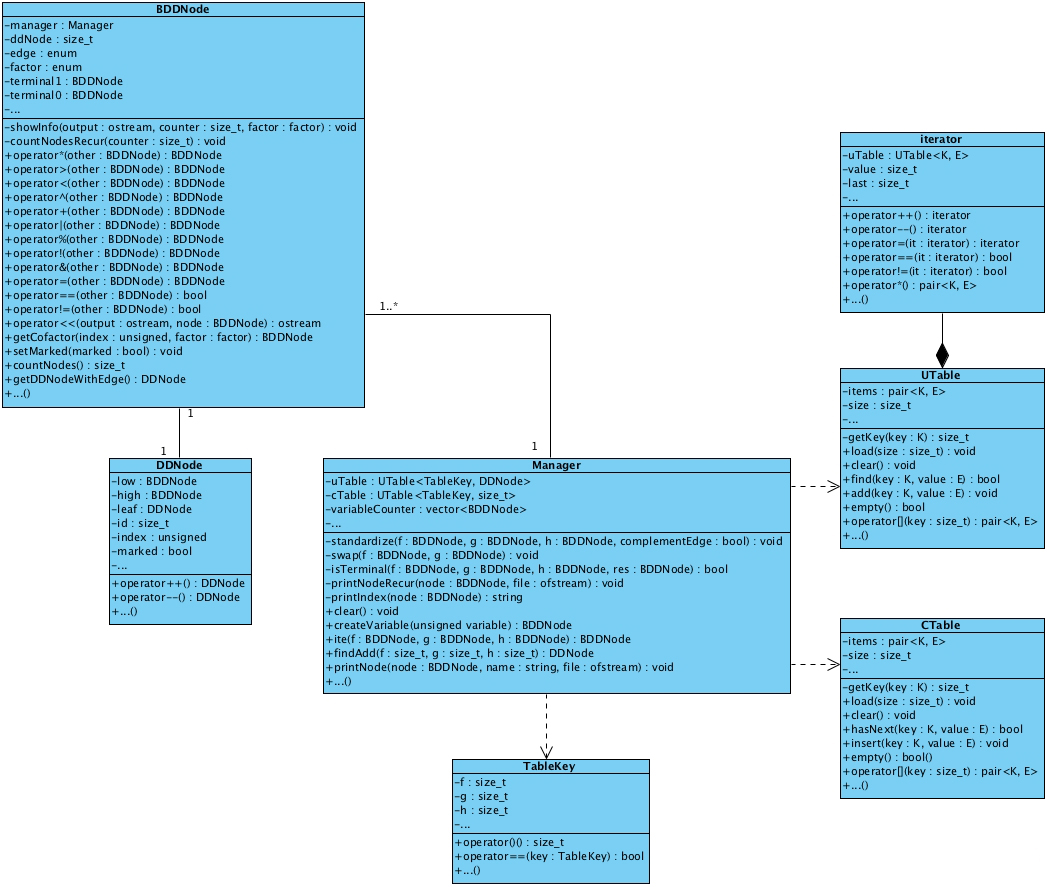
\includegraphics[scale=0.4]{./img/class}
	\caption[Zusammenspiel der Objekte im Paket]{Zusammenspiel der Objekte im Paket}
	\label{fig:class}
\end{figure}
\noindent
\textbf{Hinweis}: Aufgrund der besseren Übersichtlichkeit wurde auf die Aufführung der Konstruktoren, Destruktoren, Akzessoren und Kennzeichnung, ob eine Adresse oder Wert übergeben wird, verzichtet.\\\\
Der Programmablauf passiert phasenweise und die \texttt{load}-Methoden sind dazu da, die jeweiligen Objekte in einen endgültigen Zustand zu versetzen. Für die Tabellen wie die \texttt{CTable} oder \texttt{UTable} bedeutet es somit, dass dadurch Speicher allokiert wird. Anderseits sorgen die \texttt{clear}-Methoden dafür, dass der Speicher korrekt freigegeben sowie der Referenzzähler \texttt{id} der Klasse \texttt{DDNode} verringert wird und steht daher in einem unmittelbaren Zusammenhang zur beschrieben Speicherverwaltung (siehe Kapitel \ref{sec:speicherbereinigung} auf Seite \pageref{sec:speicherbereinigung}). Grundsätzlich greift der \texttt{Manager} also bei dessen Initialisierung auf die \texttt{CTable} sowie \texttt{UTable} zu und reserviert den angegebenen Speicher bezüglich der Knoten. Zudem werden die angegebenen Variablen in einem Vektor gespeichert, wobei die Anzahl in \texttt{variableCounter} festgehalten wird. Die damit verbundene Klasse \texttt{BDDNode} bietet Operationen wie z.\,B. die Konjunktion an, die zur Ausführung an den \texttt{Manager} für die Synthese weitergeleitet werden. Weiterhin besitzt der \texttt{BDDNode} wiederum aufgrund der automatischen Speicherbereinigung eine bidirektionale Beziehung zu einem \texttt{DDNode}, der im Unterschied dazu die jeweiligen Attribute hält. Dadurch wird es ermöglicht, den Referenzzähler \texttt{id} der Klasse \texttt{DDNode} auch automatisch zu dekrementieren, weil dieser durch den \texttt{BDDNode} eingehüllt wird. An dieser Stelle sei erwähnt, dass keine sog. \emph{Smart-Pointer} aus C++ dafür verwendet werden können, weil es keine Möglichkeit gibt, auf die Bits des Zeigers zuzugreifen. Knoten, deren \texttt{id = 0} ist, werden nicht mehr benötigt und können gelöscht werden, weshalb die innere Klasse \texttt{iterator} existiert, der eine Komposition zur Klasse \texttt{UTable} darstellt. Es können somit also Knoten in der \texttt{UTable} durchlaufen werden, um festzustellen, welche Knoten noch valide sind. Darüber hinaus wird die Klasse \texttt{TableKey} vom \texttt{Manager} dazu benutzt, um Schlüssel für deren Zugriff in der Hashtabelle über ein Modulo-Verfahren (siehe Kapitel \ref{sec:mod} auf Seite \pageref{sec:mod}) zu generieren. Es gilt dabei, dass Schlüssel (Tripel) auf Knoten in Form von Paaren abgebildet werden. Sollte bezüglich der \texttt{UTable} eine Kollision bei \texttt{add} auftreten, so wird der jeweilige Knoten in eine Überläuferliste bzw. einen gemeinsamen Slot eines Vektors abgelegt. Insgesamt basiert das Paket daher auf Indizes anstelle von Zeigern, da keine Zeiger auf Nachfolger bestehen und der Zugriff über Slots mittels \texttt{operator[]()} geregelt wird. Sollte nämlich ein 64-Bit System vorliegen, so beträgt die Größe eines Zeigers 64 anstatt 32 Bits. Um diesen Overhead bei 64-bit Rechnern zu reduzieren, können anstelle von Zeigern Integer-Indizes verwendet werden, um Knoten zu referenzieren. Letztendlich sei darauf hingewiesen, dass zur Repräsentation ganzer Zahlen der Datentyp \texttt{size\_t} verwendet wird, da bei dieser Applikation mit Speichergrenzen gearbeitet wird. Somit wird garantiert, dass sowohl auf 32- als auch 64 bit Systemen genug Kapazität zur Verfügung steht, um die angeforderten Knoten zu repräsentieren. Konkret betrachtet, steht dieser Datentyp für einen primitiven Datentypen. Wenn jedoch direkt ein primitiver Datentyp verwendet werden würde, so kann die Performanz auf manchen Systemen schlechter sein. Der Grund hierfür liegt darin, dass mehr Maschineninstruktionen bestehen würden \cite{l2015}.\\
Ein Beispiel für eine Programmausführung sowie dessen Ausgabe in Form einer Visualisierung ist im Anhang auf Seite \pageref{sec:program} zu finden. Zur Darstellung der Graphen wird in dem Zusammenhang eine Beschreibungssprache für Graphen (DOT) \cite{gkn2015} benutzt. Sämtlicher Quellcode bezüglich der entwickelten abstrakten Datentypen (ADTs) -- der im Zusammenhang mit den dazugehörigen erläuterten Konstrukten steht -- wird in den nachfolgenden Kapiteln beschrieben und erläutert.
\subsection{Gemeinsame Darstellung mehrerer Funktionen}
\label{sec:sbdds}
In Kapitel \ref{sec:bdd_grundlagen} auf Seite \pageref{sec:bdd_grundlagen} sind aufgrund der Einfachheit Boolesche Funktionen in unterschiedlichen BDDs repräsentiert worden. In einem BDD können jedoch auch mehrere Funktionen dargestellt werden, womit es verschiedene Startknoten gibt, was als SBDD bezeichnet wird. Hierzu soll das folgende Beispiel in Form einer Abbildung \ref{fig:sbdd} diesen Zusammenhang verdeutlichen:
\begin{figure}[bth]
	\centering
	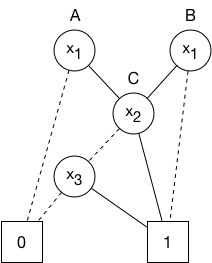
\includegraphics[scale=0.5]{./img/shared}
	\caption[Beispiel eines SBDDs]{Beispiel eines SBDDs}
	\label{fig:sbdd}
\end{figure}\\
\noindent
Der Knoten $A$ repräsentiert hier die Funktion $f_A(x_1, x_2, x_3) = x_1(x_2 + x_3)$, hingegen stellen die Knoten $B$ und $C$ die Funktionen $f_B(x_1, x_2, x_3) = x_1'(x_2+x_3)$ sowie $f_C(x_2, x_3)=x_2 + x_3$ dar.\\ 
Ein SBDD ist somit eine Ansammlung von OBDD-Knoten, die dieselbe Variablenordnung besitzen. Darüber hinaus können mehrere Funktionen gemeinsame OBDD-Knoten haben. Eine Folge daraus ist, dass Speicherplatz gespart werden kann, womit dem Hauptproblem von BDDs (siehe Kapitel \ref{sec:implementierung} auf Seite \pageref{sec:implementierung}) entgegengewirkt wird \cite{miy1990}. Zudem können aber auch mehrfach identische Berechnungen verhindert werden, was in Kapitel \ref{sec:utable} ab Seite \pageref{sec:utable} genauer erläutert wird. Im weiteren Verlauf werden daher nur noch SBDDs betrachtet.

\subsection{Der ROBDD-Knoten}
\label{sec:knoten}
Für die Implementierung der Knoten ist ein wichtiger Faktor, dass Anwendungen für ROBDDs gewöhnlicherweise mit Millionen von Instanzen davon zur Laufzeit arbeiten. Daher müssen Knoten so kompakt wie möglich realisiert werden.\\
Eine der wichtigsten Eigenschaften für die Implementierung von OBDDs ist die Eindeutigkeit in Form von ROBDDs, die in Kapitel \ref{sec:ordnung} auf Seite \pageref{sec:ordnung} beschrieben ist. Damit zusammenhängend stellt jeder Knoten genau eine Boolesche Formel mit den Variablen dar, die für die Beschriftung von Subknoten zuständig sind. Wenn nun ein Knoten $v$ in einem ROBDD die Beschriftung $l(f)$ und die \glqq Kinder\grqq{} $g, h$ besitzt, so wird der Knoten $v$ mit $ite(f,g,h)$ (siehe Code \ref{lst:ite} auf Seite \pageref{lst:ite}) als eindeutig bezeichnet. Der damit verbundene Einsatz einer Unique-Table wird in Kapitel \ref{sec:utable} auf Seite \pageref{sec:utable} erläutert. Der ADT eines Knotens benötigt also einen Verweis auf sein low-Kind \texttt{low} und high-Kind \texttt{high} sowie eine Variablenmarkierung \texttt{index}, die für eine Synthese benötigt wird, um zu einem Knoten aufgrund der Referenzen anderer zu gelangen.\\
Weiterhin ist es wichtig, einen Referenzzähler \texttt{id} einzusetzen, um sich die Anzahl der Verweise auf einen Knoten zu merken. Dadurch kann dann entschieden werden, ob ein Knoten nicht mehr benötigt wird, um dann den dazu reservierten Speicher freizugeben (siehe Kapitel \ref{sec:speicherbereinigung} auf Seite \pageref{sec:speicherbereinigung}).\\
Um die Verwaltung der Unique-Table zu unterstützen bzw. deren Speicherbedarf zu reduzieren, ist außerdem ein Verweis zur Referenzierung eines Knotennachfolgers bezüglich der Überläuferliste notwendig. Wie bereits in Kapitel \ref{sec:implementierung} auf Seite \pageref{sec:implementierung} erwähnt, wird dieser Mechanismus direkt in der Unique-Table realisiert, sodass sich verkettete Überläufer in einem Slot bzw. Vektor befinden. Dadurch liegen die Knoten hinsichtlich des Speichers eng beieinander und durch ihre Position wird Zeiger-Arithmetik möglich, womit ein konstanter Zugriff auf alle Felder besteht. Zudem entfällt ein Attribut im Knoten, der auf den Nachfolger zeigen würde. Dadurch werden die Unique-Table als auch der Knoten miteinander kombiniert, was in Kapitel \ref{sec:utable} auf Seite \pageref{sec:utableBdd} erläutert wird. Das zugrunde liegende Prinzip der Kollisionsbehandlung wird wiederum in Kapitel \ref{sec:verkettung} auf Seite \pageref{sec:verkettung} erläutert.\\
Das Attribut \texttt{marked} wird bei der Traversierung durch den Graphen benötigt und von Methoden wie z.\,B. \texttt{printNode} des Managers verwendet, um das BDD zu visualisieren. Dadurch wird wiederum ausgeschlossen, dass Knoten doppelt gezählt werden.\\
Insgesamt gesehen, darf ein Platzbedarf von approximiert $22$ Bytes angenommen werden, wenn die Anzahl möglicher Variablen auf $2^{16}$ begrenzt ist \cite[S.81-82]{h2002}. Dementsprechend gelten zwei Bytes für die Markierung und jeweils vier Bytes für weitere Daten, wobei die genaue Zusammenstellung ebenfalls in Kapitel \ref{sec:utableBdd} auf Seite \pageref{sec:utableBdd} erläutert wird.

\subsection{Synthese von ROBDDs}
\label{sec:synthese}
Eine \emph{Synthese} umfasst die Berechnung der Darstellung einer Booleschen Funktion anhand bereits vorhandener Darstellungen. Dazu werden BDDs i.\,d.\,R. erzeugt, indem bestehende BDDs \glqq Bottom-up\grqq{} miteinander kombiniert werden. Zu Beginn werden daher primitive BDDs angelegt (beginnend bei den Blättern), die zur Darstellung von Funktionen $f = x_i \forall x_i$, die als Entscheidungsvariablen vorkommen, dienen. Diese werden dann dementsprechend kombiniert und verknüpft, d.\,h. synthetisiert, um die Repräsentation der gewünschten Booleschen Funktion zu erhalten.

\subsubsection{Der ITE-Operator}
\label{sec:ite}
Der ITE-Operator ist der Kern des Paketes und stellt einen Universal-Syntheseoperator dar. Bezüglich der Namensgebung steht ITE für \glqq If $f$ Then $g$ Else $h$\grqq{}:
\newpage
\begin{figure}[bth]
	\centering
	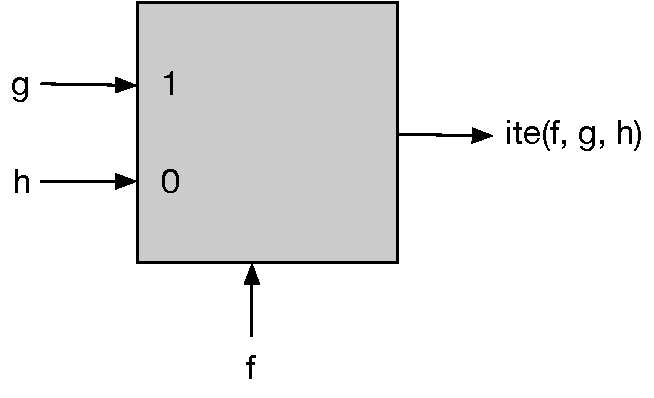
\includegraphics[scale=0.5]{./img/ite2}
	\caption[Visualisierung des ITE-Operators]{Visualisierung des ITE-Operators}
	\label{fig:iteo}
\end{figure}
\noindent
Gemäß der Abbildung \ref{fig:iteo} benötigt der Operator also drei Operanden, um die Boolesche Funktion $ite(f, g, h) = f \cdot g + f' \cdot h$ berechnen zu können. Ist $f$ eine Entscheidungsvariable, so entspricht diese Darstellung genau der Shannon-Zerlegung (siehe Kapitel \ref{sec:bdd} auf Seite \pageref{sec:bdd}). Boolesche Funktionen können also mittels eines Aufrufs des ITE-Operators geschrieben werden.\\
In einem BDD werden Boolesche Operatoren realisiert. Alle Booleschen Operatoren aus der Menge $\mathbb{B_1}$ und $\mathbb{B_2}$ (bei mehreren Variablen muss explizit eine Funktionskonkatenation stattfinden) können auf diesen ternären Operator direkt zurückgeführt werden \cite{cm1994}, was die folgende Tabelle \ref{tab:ite} verdeutlicht:
\begin{table}[bth]
	\centering
	\caption{ITE Operator}
	\label{tab:ite}
	\begin{tabular}{ | l | l | l | l | }
		\hline
		\textbf{Nummer} & \textbf{Name} & \textbf{Ausdruck} & \textbf{Äquivalente Form} \\ \hline
		$0000$ & $0$ & $0$ & $0$ \\ \hline
		$0001$ & $and(f,g)$ & $fg$ & $ite(f,g,0)$ \\ \hline
		$0010$ & $f > g$ & $f\neg g$ & $ite(f,\neg g,0)$ \\ \hline
		$0011$ & $f$ & $f$ & $f$ \\ \hline
		$0100$ & $f < g$ & $\neg fg$ & $ite(f,0,g)$ \\ \hline
		$0101$ & $g$ & $g$ & $g$ \\ \hline
		$0110$ & $xor(f,g)$ & $f \oplus g$ & $ite(f,\neg g,g)$ \\ \hline
		$0111$ & $or(f,g)$ & $f+g$ & $ite(f,1,g)$ \\ \hline
		$1000$ & $nor(f,g)$ & $\neg (f+g)$ & $ite(f,0,\neg g)$ \\ \hline
		$1001$ & $xnor(f,g)$ & $\neg (f \oplus g)$ & $ite(f,g,\neg g)$ \\ \hline
		$1010$ & $not(g)$ & $\neg g$ & $ite(g,0,1)$ \\ \hline
		$1011$ & $f \geq g$ & $f + \neg g$ & $ite(f,1,\neg g)$ \\ \hline
		$1100$ & $not(f)$ & $\neg f$ & $ite(f,0,1)$ \\ \hline
		$1101$ & $f \leq g$ & $\neg f + g$ & $ite(f,g,1)$ \\ \hline
		$1110$ & $nand(f,g)$ & $\neg (fg)$ & $ite(f,\neg g,1)$ \\ \hline
		$1111$ & $1$ & $1$ & $1$ \\ \hline
	\end{tabular}
\end{table}\\
\noindent
So gilt bspw. $ite(f, g, 0) = f \cdot g + f' \cdot 0 = f \cdot g$ für die Konjunktion, wobei ein derartiger Aufruf direkt bei den Operatorüberladungen wie z.\,B. \texttt{operator*()} im \texttt{BDDNode} (siehe Abbildung \ref{fig:class} auf Seite \pageref{fig:class}) erfolgen kann.\\
Die Argumente für den ITE-Operator können dazu automatisch aus der rekursiven Formulierung infolge der Shannon-Zerlegung erhalten werden. Sei also $v$ die top-Variable von $f, g, h$. Dann gilt gemäß Shannon-Zerlegung und Anwendung des ITE-Operators:\\
\begin{equation*}
	\begin{split}
		ite(f, g, h) &= f \cdot g + f' \cdot h \\
		&= v \cdot (f \cdot g + f' \cdot h)_v + v' \cdot (f \cdot g + f' \cdot h)_{v'}\\
		&= v \cdot (f_v \cdot g_v + f'_v \cdot h_v) + v' \cdot (f_{v'} \cdot g_{v'} + f'_{v'} \cdot h_{v'})\\
		&= (v, ite(f_v, g_v, h_v), ite(f_{v'}, g_{v'}, h_{v'}))
	\end{split}
\end{equation*}
Jeder Knoten speichert also ein Tripel mit einer Variablen $v$, an welcher er zerlegt wurde sowie zwei \glqq Kindern\grqq{}, die sich rekursiv aus einem ITE-Aufruf der Kofaktoren ergeben. Die Knoten werden also durch $(f, g, h)$ eindeutig bezeichnet. Die Kofaktoren von $f, g, h$ nach $v$ können dazu weiterhin bestimmt werden. Sei dazu $f$ ein Knoten, wobei $f = (r, t, e), v \leq r$ ist. Dann gilt:\\
\begin{equation*} 
f_v = \begin{cases} 
f & \text{für } v < r \\ 
t & \text{für } v = r
\end{cases} 
\end{equation*}
\begin{equation*}
f_{v'} = \begin{cases} 
f & \text{für } v < r \\ 
e & \text{für } v = r
\end{cases} 
\end{equation*}
Sollte $v < u$ gelten, so kommt die Variable $v$ demnach nicht in $f$ vor, da $v$ die top-Variable von $f$ ist. Folgender Code \ref{lst:cofactor} verdeutlicht die Berechnung des Kofaktors:
\lstset{language=xml}
\begin{lstlisting}[frame=htrbl, caption={Implementierung von {\ttfamily getCofactor}}, label={lst:cofactor}]
program getCofactor()
  input: OBDD f, Variable index, Factor factor (high/low)
  output: Kofaktor des jeweiligen Operanden
  t := BDDNode
  e := BDDNode
  edgeF := Kante von f
  if ( index > index(f) ) then
    return f
  end if
  if ( index = index(f) ) then
    if ( high(factor) ) then
      return isComplementEdge(f) ? !high(f) : high(f)
    else 
      return isComplementEdge(f) ? !Low(f) : low(f)
  end if
  t := ( high(factor) ) ? getCofactor(high(f), index, high) :
    getCofactor(low(f), index, low)
  e := ( high(factor) ) ? getCofactor(low(f), index, high) : 
    getCofactor(low(f), index, low)
  if (t = e) then
    return isComplementEdge(f) ? !t : t
  end if
  if ( isComplementEdge(f) ^ isComplementEdge(t) ) then
    edgeF := complement
  else
    edgeF := regular
  end if
  if ( isComplementEdge(t) ) then
    t := !t
    e := !e
  end if
  return BDDNode(index(f), getDDNode(t), getDDNode(e), edgeF)
end program
\end{lstlisting}
Für eine komplementäre Kante (siehe Kapitel \ref{sec:complementEdges}) auf Seite \pageref{sec:complementEdges}) erfolgt also bspw. die Berechnung von $f_{x_{i=0}} = f(\dots, x_{i-1}, 0, x_{i+1}, \dots)$ im Rahmen einer Traversierung, die linear durch das ROBDD beschränkt ist, wobei für jeweils eine Variable eine konstante Funktion eingesetzt wird.\\
Hinsichtlich des Verfahrens wird zunächst das ursprüngliche ROBDD kopiert, wobei jede Kante, die einen Knoten $f$ mit $index(f) = x_i$ referenziert, durch eine Kante auf $low(f)$ bzw. $high(f)$ infolge der Reduktionsregeln ersetzt wird. Der Kofaktor nach $x_i$ eines Knotens $f$ entspricht also der Low-Kante, wenn dieser Knoten mit $x_i$ markiert ist. Ansonsten gilt der Knoten $index(f), low(f)_{x_i=0'}, high(f)_{x_i=0}$. Wie bereits erwähnt, ist der Kofaktor einer Variable oftmals die Wurzelmarkierung. In diesem Fall entspricht die Lösung einem der beiden \glqq Kinder\grqq{} und es besteht lediglich eine konstante Laufzeit \cite{g2002}. Die jeweiligen Abfragen \texttt{isComplementEdge()} kennzeichnen weiterhin eine Überprüfung, ob eine komplementäre Kante (siehe Kapitel \ref{sec:complementEdges} auf Seite \pageref{sec:complementEdges}) vorliegt. Damit die Not-Operation in konstanter Laufzeit erfolgen kann, wird in dem SBDD auch die jeweilige Negation des BDDs dargestellt. Daher müssen also auch komplementäre Kanten passiert werden können, wozu diese Abfragen dienen.\\
Der ITE-Operator ist also insgesamt mit der Shannon-Dekomposition verträglich. In Kapitel \ref{sec:operationen} auf Seite \pageref{sec:operationen} wurde im Hinblick auf die Operationen ein Vergleich zu anderen Darstellungen von Booleschen Funktionen gemacht, was bezüglich der Kofaktor-Berechnung ebenfalls in der Tabelle \ref{tab:cofactor} auf Seite \pageref{tab:cofactor} betrachtet wird \cite{m2007}:
\newpage
\begin{table}[bth]
	\centering
	\caption{Vergleich der Kofaktor-Berechnung für Darstellungen}
	\label{tab:cofactor}
	\begin{tabular}{ | l | p{10cm} | }
		\hline
		\textbf{Darstellung} & \textbf{Beschreibung} \\ \hline
		Wahrheitstafel & Die Laufzeit ist proportional zu $2^n$, d.\,h. linear in der Größe zur Wahrheitstafel.\\ \hline
		Boolesche Ausdrücke & Es wird zunächst der Operatorbaum (siehe Kapitel \ref{sec:bAusdruecke} auf Seite \pageref{sec:bAusdruecke}) kopiert. Anschließend erfolgt eine Ersetzung der mit der Variablen markierten Blätter durch die entsprechende Konstante. Zuletzt wird eine Reduzierung des Baumes \glqq Bottom-up\grqq{} vorgenommen. Insgesamt ist das Verfahren daher polynomiell beschränkt. \\ \hline
		DNF & Die entsprechenden Literale werden ersetzt, anschließend erfolgt eine Reduzierung der DNF. Offensichtlich gilt eine polynomielle Laufzeit. \\ \hline
		KNF & Auch hier werden die entsprechenden Literale ersetzt, anschließend erfolgt eine Reduzierung der KNF. Offensichtlich gilt ebenfalls eine polynomielle Laufzeit. \\ \hline
		Schaltkreise & Die Komplexität entspricht den Booleschen Ausdrücken. \\ \hline
	\end{tabular}
\end{table}
\noindent 
Alle ein- und zweistelligen Booleschen Funktionen können direkt durch verschiedene Aufrufe des ITE-Operators geschrieben werden, wodurch die Implementierung deutlich vereinfacht wird \cite{brb2007}. Dieser universelle Operator wird also insbesondere dafür verwendet, um OBDDs zu konstruieren und kann wie folgt rekursiv über die angesprochenen Kofaktoren (siehe Code \ref{lst:cofactor} auf Seite \pageref{lst:cofactor}) der Operanden implementiert werden:
\lstset{language=xml}
\begin{lstlisting}[frame=htrbl, caption={Implementierung von {\ttfamily ite}}, label={lst:ite}]
program ite()
  input: f, g, h (OBDDs)
  output: OBDD ite(f, g, h)
  cT := Computed-Table
  uT := Unique-Table
  top := top-Variable
  resT, resC, f1, g1, h1, f0, g0, h0, t, e := BDDNode
  node := DDNode
  key := TableKey
  complementEdge := false
  standardize(f, g, h, complementEdge)
  if ( isTerminal(f, g, h, resT) ) then
    if (complementEdge = true) then
      resT := !resT
      return resT
    end if
  end if
  key := getKey( getDDNode(f), getDDNode(g), getDDNode(h) )
  if ( cT.hasNext(key, resC) ) then 
    if (complementEdge = true) then
      resC := resC ^ getComplementEdge()
    end if
    return resC
  end if
  top := index(f)
  if (index(g) > top) then
    top := index(g)
  end if
  if (index(h) > top) then
    top := index(h)
  end if
  f1 := getCofactor(f, top, high)
  g1 := getCofactor(g, top, high)
  h1 := getCofactor(h, top, high)
  f0 := getCofactor(f, top, low)
  g0 := getCofactor(g, top, low)
  h0 := getCofactor(h, top, low)
  t := ite(f1, g1, h1)
  e := ite(f0, g0, h0)
  if (t = e) then
    if (complementEdge = true) then
      t := !t
      return t
    end if
  end if
  node := uT.findAdd( top, getDDNode(t), getDDNode(e) )
  resC := node
  cT.insert(key, resC)
  if (complementEdge = true) then 
    resC = resC ^ getComplementEdge()
  end if
  return resC
end program
\end{lstlisting}
Die Konzepte der Computed-Table und Unique-Table werden in den Kapiteln \ref{sec:ctable} ab Seite \pageref{sec:ctable} sowie \ref{sec:utable} ab Seite \pageref{sec:utable} genauestens erläutert.\\
Zunächst einmal wird der Aufruf standardisiert (Z. 11), d.\,h. Kombinationen, die zum gleichen Ergebnis führen, werden in Äquivalenzklassen zusammengefasst, wobei ein Repräsentant ausgewählt wird. Diese Technik wird in Kapitel \ref{sec:standard} auf Seite \pageref{sec:standard} erläutert.\\
Danach wird auf die Terminierung des Verfahrens geprüft (Z. 12-17), was z.\,B. bei $ite(1, f, g) = ite(0, g, f) = ite(f, 1, 0) = f$ der Fall wäre. In einem solchen Fall kann das Ergebnis unmittelbar zurückgegeben werden.\\
Sollte sich der mit diesen Parametern berechnete OBDD-Knoten noch in der Computed-Table befinden, so kann ebenfalls direkt dieser Knoten als Ergebnis zurückgegeben werden (Z. 18-24). Somit werden weitere Aufrufe in diesem Rekursionsschritt gespart.\\
Ansonsten werden zwei Teilprobleme \texttt{t, e} für die Kofaktoren der Operanden erzeugt, wobei die Wurzelmarkierung $x_i$ ausgewählt wird, die in der Ordnung zuerst vorkommt. Dabei gilt, dass der höhere Index zuerst abgefragt wird (Z. 25-31).\\
Somit können die dazugehörigen Kofaktor-Berechnungen (siehe Code \ref{lst:cofactor} auf Seite \pageref{lst:cofactor}) für diese Variable in $O(1)$ erfolgen, da ein Kofaktor für einen Operanden eine Selbstreferenz liefert (wenn der Operand nicht von $x_i$ abhängt) oder einem der \glqq Kinder\grqq{} entspricht (Z. 32-37). Weiterhin wird diese Steigerung der Performanz durch die Festlegung einer identischen Variablenordnung für alle Operanden ermöglicht \cite[S.37-38]{h2002}.\\
Nachdem beide Teilprobleme berechnet worden sind (Z. 38-39), erfolgt eine Überprüfung auf Isomorphie (Z. 40-45), was bezüglich SBDDs durch einen Vergleich der beiden Wurzeln von \texttt{t, e} in $O(1)$ erfolgt (siehe Kapitel \ref{sec:verifikation} auf Seite \pageref{sec:verifikation}). Es ist also die Anwendung der Isomorphie-Regel (siehe Abbildung \ref{fig:reduktionen} auf Seite \pageref{fig:reduktionen}) erforderlich. Sollte keine Isomorphie bestehen, so entspricht das Ergebnis daher einem Wurzelknoten $r$ mit der Markierung $x_i$ sowie den \glqq Kindern\grqq{} $low(r) = e$ und $high(r) = t$. Die Wurzel könnte allerdings bereits existieren, womit die Redundanzregel greifen würde. Daher soll in $O(1)$ ein solcher Fall vermieden werden. Der Knoten sollte also nur erstellt werden, wenn er noch nicht existiert.\\
Zur Speicherung bereits vorhandener Ergebnisse wird dementsprechend die Unique-Table (Z. 46) benutzt. Die Funktion \texttt{findAdd} (siehe Code \ref{lst:findAdd} auf Seite \pageref{lst:findAdd}) prüft, ob ein vorgegebenes Tripel bereits in OBDD-Knoten realisiert ist. Im positiven Fall gibt sie eine Referenz auf den Knoten zurück, ansonsten wird  mittels \texttt{add} ein neuer Knoten erzeugt und darauf ein Verweis zurückgeliefert. Der Vorgang der jeweiligen Überprüfung sowie Erstellung eines Knoten wird häufig auch in einer Funktion \texttt{mk} zusammengefasst.\\
Die anschließende Funktion \texttt{insert} (Z. 47-48) fügt das wiederum berechnete Teilproblem in die Computed-Table ein. Ohne diesen Cache würde der obige Algorithmus auch -- vom Wurzelknoten ausgehend -- alle Wege bis zu $0, 1$ durchlaufen, wobei die zusammengefassten Teilgraphen allerdings mehrmals betrachtet werden würden. Sollten durch den Einsatz einer Computed-Table wiederum alle bereits berechneten Ergebnisse gespeichert werden, dann wird der ITE-Algorithmus für jede Knotenkombination der drei OBDDs $f, g, h$ aufgerufen.\\
Damit die Negation in $O(1)$ ermittelt werden kann, erfolgt zusätzlich die Berechnung komplementärer Kanten, wobei die Standardisierung die binäre Variable\\\texttt{complementEdge} dazu verändern kann. Mittels \texttt{getComplementEdge} (Z. 49-51) passiert wiederum ein Zugriff auf eine solche Kante. Wenn demnach eine komplementäre Kante vorliegt, so muss das jeweilige Ergebnis negiert werden. Das Prinzip dahinter wird in Kapitel \ref{sec:complementEdges} auf Seite \pageref{sec:complementEdges} erläutert.\\ 
Offensichtlich unterliegt der Algorithmus also dem \emph{Divide and Conquer}-Prinzip, d.\,h. ein Problem wird in Teilprobleme aufgeteilt, anschließend werden diese einzeln gelöst und zusammengefasst. Auf dieses Verfahren bezogen, ist somit jeder Operator von Kofaktoren demnach ein Kofaktor von Operatoren.\\
Die Funktionsweise zur Synthese einer Funktion des ITE-Algorithmus soll nun anhand der Abbildung \ref{fig:ite} verdeutlicht werden:
\begin{figure}[bth]
	\centering
	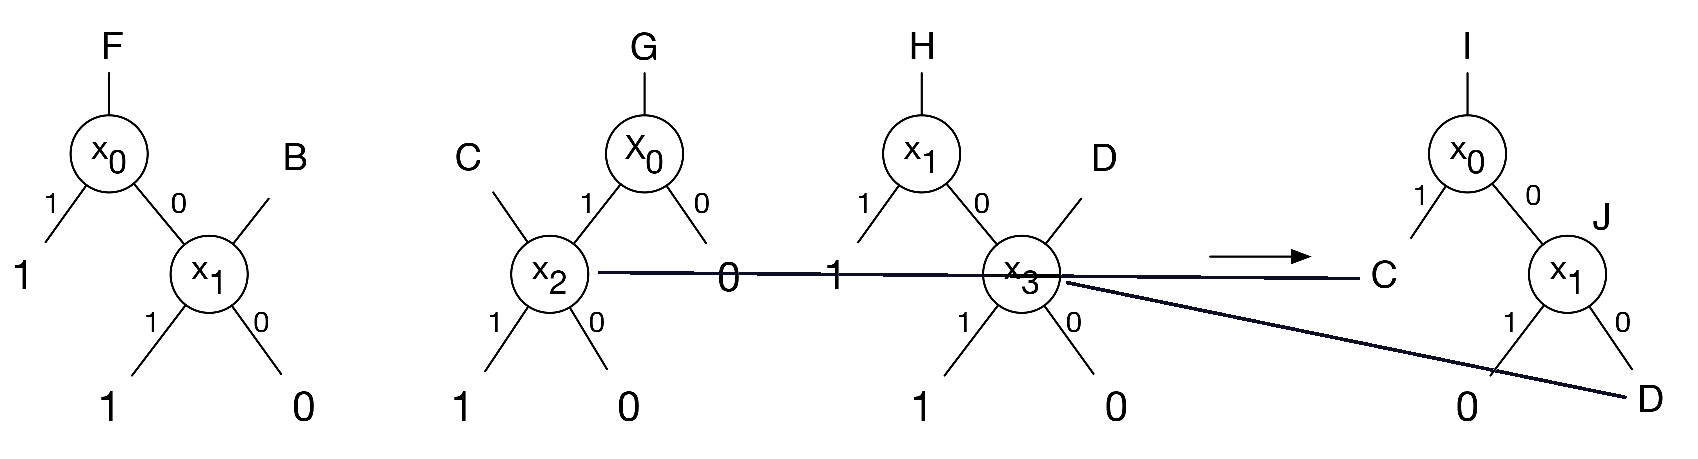
\includegraphics[scale=0.5]{./img/ite}
	\caption[Beispiel des ITE-Algorithmus]{Beispiel des ITE-Algorithmus}
	\label{fig:ite}
\end{figure}\\
Es sind verschiedene BDDs von unterschiedlichen Booleschen Funktionen dargestellt. Dabei sind $F, G, H, I, J, B, C, D$ als Zeiger zu verstehen. Der durch den Aufruf\\ $ite(F, G, H)$ berechnete OBDD $I$ gemäß Abbildung \ref{fig:ite} ergibt sich nachstehend:
\begin{equation*}
\begin{split}
I &= ite(F,G,H)\\
  &= (x_0, ite(F_{x_0}, G_{x_0}, H_{x_0}), ite(F_{x_0'}, G_{x_0'}, H_{x_0'}))\\
  &= (x_0, ite(1, C, H), ite(B, 0, H))\\
  &= (x_0, C, (x_1, ite(B_{x_1}, 0_{x_1}, H_{x_1}), ite(B_{x_1'}, 0_{x_1'}, H_{x_1'}))\\
  &= (x_0, C, (x_1, ite(1, 0, 1), ite(0, 0, D)))\\
  &= (x_0, C, (x_1, 0, D))\\
  &= (x_0, C, J)
\end{split}
\end{equation*}
Wenn z.\,B. $F = x_0+x_1$, $G = x_0 \cdot x_2$ und $H = x_1 + x_3$ aus $\mathbb{B}_4$ angenommen werden, so ergibt sich bezüglich dem ITE-Operator hinsichtlich einer Überprüfung $ite(F,G,H) = (x_0+x_1)(x_0x_2) + x_0'x_1'(x_1+x_3) = x_0x_2+x_0'x_1'x_3$.\\
Zu jedem Tripel $(f,g,h)$ existieren also weitere Tripel $(f',g',h')$, sodass $ite(f,g,h) = ite(f',g',h')$, obwohl mindestens einer der Operatoren verschieden ist. Wenn diese verschiedenen Paare mit dem gleichen Ergebnis auf einen eindeutigen Repräsentanten abgebildet werden, so können mithilfe einer Computed-Table zusätzliche ITE-Aufrufe gespart werden.\\
Das Einfügen bzw. Ermitteln von Knoten in der Computed-Table bzw. Unique-Table benötigt eine konstante Zeit (siehe Kapitel \ref{sec:ctable} ab Seite \pageref{sec:ctable} sowie \ref{sec:utable} ab Seite \pageref{sec:utable}). Aufgrund dessen beträgt die Zeit- und Speicherkomplexität des ITE-Algorithmus $O(|f| \cdot |g| \cdot |h|)$ (kubisch), weil der Operator höchstens einmal für jede Kombination von Knoten in $f, g, h$ aufgerufen werden kann. Ohne die jeweiligen Tabellen würde sich der Algorithmus ansonsten für die Lösung jedes Teilproblems zweifach rekursiv für maximal jede Variable aufrufen, was eine exponentielle Laufzeit in der Anzahl der Variablen bedeuten würde.\\
Meistens ist es ausreichend, zu berechnen, ob ein ITE-Aufruf eine konstante Funktion liefert, um bereits frühzeitig für eine Terminierung zu sorgen. Soll bspw. $f \Rightarrow g$ überprüft werden, so genügt es zu zeigen, dass $\neg f+g$ eine Tautologie (siehe Kapitel \ref{sec:tautologietest} auf Seite \pageref{sec:tautologietest}) ist, indem es mithilfe eines adaptierten ITE-Algorithmus berechnet wird. Das Ergebnis ist uninteressant, wenn es nicht konstant ist. Der folgende Algorithmus \ref{lst:iteConstant} verdeutlicht die damit zusammenhängende Modifizierung des ITE-Algorithmus (siehe Code \ref{lst:ite} auf Seite \pageref{lst:ite}):
\lstset{language=xml}
\begin{lstlisting}[frame=htrbl, caption={Implementierung von {\ttfamily iteConstant}}, label={lst:iteConstant}]
program iteConstant()
  input: f, g, h (OBDDs)
  output: Status, ob eine konstante Funktion vorliegt
  cT := Computed-Table
  res := OBDD-Knoten
  if (terminal) then
    // 0, 1 oder NC
    return res
  else if ( res := cT.hasNext(f, g, h) )
    return NC
  else
    top := top-Variable von (f, g, h)
    t := iteConstant(f[top], g[top], h[top])
    if (t != 0 and t != 1)
      return NC
    end if
    e := iteConstant(f[top'], g[top'], h[top'])
    if (t != e) then 
      return NC
    end if
    cT.insert(hash(f, g, h), t)
  end if
end program
\end{lstlisting}
Dabei entspricht \texttt{NC} \glqq Non Constant\grqq{}, zudem wurde aufgrund der Übersichtlichkeit auf die explizite Berechnung der Kofaktoren, komplementären Kanten und Standardisierung verzichtet.\\
Eine Funktion ist also nur dann konstant, wenn beide Kofaktoren konstant und gleich sind. Andernfalls ist sie nicht konstant und der Algorithmus wird vorzeitig abgebrochen. Weiterhin ist hierbei die Nützlichkeit für die logische Implikation zu erkennen, da bspw. $f \Rightarrow g \Leftrightarrow iteConstant(f, g, 1) = 1$. Eine derartige Operation kann im Vergleich zum allgemeinen ITE-Operator durchschnittlich effizienter vollzogen werden, da keine temporären Knoten konstruiert werden müssen und dieser -- wie bereits erwähnt -- frühzeitig abgebrochen werden kann.\\
Im folgenden Abschnitt wird gezeigt, wie Knoten innerhalb der beschriebenen Synthese effizient gespeichert bzw. wiederverwendet werden können.

\subsection{Die Unique-Table (UT)}
\label{sec:utable}
Die \emph{Unique-Table} (UT) wird als Hashtabelle realisiert, womit es gelingt, eine streng kanonische Form (siehe Kapitel \ref{sec:ordnung} auf Seite \pageref{sec:ordnung}) im ROBDD zu erhalten. Im Endeffekt werden dort die Subfunktionen abgespeichert, die bereits vom BDD repräsentiert werden. Dadurch ist es möglich, beim Hinzufügen oder Berechnen neuer Funktionen, ohne großen Suchaufwand bereits vorhandene Knoten einzusetzen \cite{h2011}. Die UT sorgt also dafür, dass Isomorphien nicht auftreten können bzw. sorgt ein Vergleich der Kofaktoren (Kinder des neuen Knotens) für die Reduktion des OBDDs.\\
Mithilfe von Hashverfahren ist es möglich, Knotenzugriffe bzw. Existenzprüfungen effizient zu realisieren. Im Worst Case kann ein Hashverfahren aber auch sehr ineffizient sein, weil Kollisionen nicht gänzlich verhindert werden können (Hashfunktionen sind injektiv) und die Performanz der Operationen \emph{Einfügen}, \emph{Suchen} sowie \emph{Entfernen} maßgeblich von einem sog. Belegungsfaktor abhängt. Im Folgenden soll daher die Wahl der jeweiligen Hashfunktion. Tabellengröße und Kollisionsbehandlung diskutiert werden.

\subsubsection{Das Hashverfahren}
\label{sec:hashing}
Bei der UT spielt \emph{Hashing} als Technik eine große Rolle. Die Grundlage für Hashing bildet die Berechnung eines Index aus einem Suchwert. Dabei enthält Hashing zwei wesentliche Komponenten:
\begin{itemize}
	\item \textbf{Hashfunktion}: Bildet Objekte auf Natürliche Zahlen, sog. Hashcodes ab, die als numerische Schlüssel zur Identifikation der Objekte genutzt werden.
	\item \textbf{Hashtabelle}: Kennzeichnet eine Liste, in der Objekte eingetragen werden, wozu der Hashcode als Index genutzt wird.
\end{itemize}
Weiterhin kennzeichnet $a = \frac{n}{m}$ den sog. \emph{Belegungsfaktor}, der die Anzahl der Datensätze $n$ in das Verhältnis zur Größe der Hashtabelle $m$ setzt. Der Zugriff auf ein Element ist folglich definiert durch $O(a)$. Offensichtlich ist Hashing besonders dann effektiv, wenn $m$ im Verhältnis zu $n$ nicht zu klein ist. Werden die Hashfunktion und die Größe der Tabelle geeignet gewählt, so beträgt der Aufwand für den Zugriff nur $O(1)$, was im Folgenden diskutiert wird und in Kapitel \ref{sec:collision} auf Seite \pageref{sec:collision} genau beschrieben ist. Eine gute Hashfunktion ist demnach schnell berechenbar respektive verteilt die Datensätze nach Möglichkeit gleichmäßig auf den Speicherbereich. Weiterhin sorgt der Einsatz der UT im ITE-Algorithmus dafür, dass der Aufwand dieses Operators kubisch beschränkt ist (siehe Kapitel \ref{sec:ite} auf Seite \pageref{sec:ite}).\\
Hinsichtlich der Schlüsselwahl wird jedem Tripel $(v, g, h)$ ein Knoten zugeordnet. Jeder Knoten besitzt also einen Eintrag in der Hashtabelle. Bevor ein neuer Knoten $f = (v, g, h)$ eingefügt wird (siehe Code \ref{lst:ite} auf Seite \pageref{lst:ite}), erfolgt eine Überprüfung, ob es nicht schon einen entsprechenden Eintrag gibt. Der folgende Code \ref{lst:findAdd} verdeutlicht diese Operation:
\lstset{language=xml}
\begin{lstlisting}[frame=htrbl, caption={Implementierung von {\ttfamily findAdd}}, label={lst:findAdd}]
program findAdd()
  input: f, g, h (Adressen von Knoten)
  output: Adresse eines Knoten aus der UT
  key := TableKey
  ddNode := DDNode
  uTable := Unique-Table
  key := getKey(f, g, h)
  if ( !uTable.find(key, ddNode) ) then
    create(ddNode)
    uTable.add(key, ddNode)
  end if
  return ddNode
end program
\end{lstlisting}
Die relevante Operation hierbei, um eine dementsprechende Überprüfung zu erledigen, ist \texttt{find} und als Code \ref{lst:find} folgendermaßen aufgebaut:
\lstset{language=xml}
\begin{lstlisting}[frame=htrbl, caption={Implementierung von {\ttfamily find}}, label={lst:find}]
program find()
  input: key, value (Knoten)
  output: Status, ob es den Knoten bereits in der UT gibt
  pos := getKey(key)
  items := Vektor mit Abbildungen von Keys auf Knoten
  nodes := size(items[pos])
  for (i to nodes) do
    if (items[pos][i].first = key) then
      value := items[pos][i].second
      return true
    end if
  end for
  return false
end program
\end{lstlisting}
Wenn also bereits ein Knoten existiert, wird der Eintrag ohne Aktualisierung benutzt, ansonsten wird der jeweilige Knoten in die Hashtabelle mit aufgenommen und erhält einen Eintrag. Somit kann ein Knoten über \texttt{items[getKey(key)].push(pair(key, value))} eingetragen werden. Sollte eine Kollision auftreten, so wird der Knoten direkt als Nachfolger eingetragen.\\
Somit bildet das Tripel den Schlüssel, um auf einen Knoten zugreifen zu können. Daraus folgt, wenn $g$ und $h$ bereits eine Kanonizität vorweisen, so existiert $f$ im ROBDD unter der Voraussetzung, dass es einen Eintrag für $(v, g, h)$ gibt. Infolge der Verwendung des ITE-Operators und der UT folgt also automatisch die Kanonizität.\\
In der Praxis werden i.\,d.\,R. zwei Methoden eingesetzt \cite[S.72-73]{h2002}, nämlich das Modulo- sowie Multiplikations-Verfahren, die nun beschrieben werden, wobei ein direkter Vergleich bezüglich experimenteller Ergebnisse in Kapitel \ref{sec:ovh} auf Seite \pageref{sec:ovh} gemacht wird.

\pgraph{Das Modulo-Verfahren}
\label{sec:mod}
Bei dem \emph{Modulo-Verfahren} lautet die Hashfunktion $h(k) = k \text{ }mod\text{ } m$, wobei $k$ dem Schlüssel und $m$ der Größe der Hashtabelle entspricht, wobei $m$ für eine gute Gleichverteilung der Elemente in der Tabelle eine Primzahl sein sollte \cite{k2011}. Bezogen auf Knoten, wird $k$ durch das jeweilige Tripel $f, g, h$ ersetzt, d.\,h. es gilt die Funktion $h(f, g, h) = ( (g + h) >> f) \text{ }mod\text{ } m$. Hierbei kennzeichnet $>>$ einen bitweisen Operator bzw. Rechtsshift.\\
Wird der Divisionsblock einer Arithmetisch-logischen Einheit (ALU) des Prozessors (CPU) betrachtet, so kann festgestellt werden, dass dies eine zeitintensive Rechenoperation ist \cite[S.73]{h2002}. Hingegen können andere Operationen wie der Rechts-Shift um $i$ Stellen eingesetzt werden. Dieser entspricht dabei Divisionen mit einem Divisor $2^i$ für ein $i \in \mathbb{N}$ in Abhängigkeit zu der Wortbreite des Rechners. Für viele Eingaben ist hierbei die Wahl einer Zweierpotenz für $m$ nicht geeignet, da die höherwertigen Bits bei den Hash-Berechnungen ignoriert werden, was zu einer Ungleichverteilung der Schlüssel führt. Wird hingegen $m$ als Primzahl derartig festgelegt, dass keine Mersenne-Primzahl der Form $2^i - 1$ besteht, so gibt es eine geringe Anzahl von zu erwarteten Kollisionen bei vielen Eingabeverteilungen \cite[S.231]{clrs2001}.

\pgraph{Das Multiplikations-Verfahren}
\label{sec:mul}
Das \emph{Multiplikations-Verfahren} berechnet durch die Funktion $h(k) = \lfloor m \cdot (kx- \lfloor kx \rfloor) \rfloor$ die Hashadresse, wobei $k$ den Schlüssel und $x :=   \frac{(\sqrt{5}-1)}{2}$ eine irrationale Zahl sowie $m$ die Größe der Hashtabelle kennzeichnet. Um eine gleichmäßige Verteilung der Datensätze zu erreichen, wird $x$ als Kehrwert des \emph{goldenen Schnittes} gewählt \cite{ow1990}.\\
Innerhalb der ALU wird die Fließkommazahl zur Multiplikation verwendet, um irrationale Zahlen zu verarbeiten \cite[S.74]{h2002}. Auch diese Methode ist zeitintensiv, jedoch können ganze Zahlen im Rechner als Bruchzahlen mit einem Dezimalpunkt vor der höchstwertigen Ziffer betrachtet werden, wobei für $m$ dann eine Zweierpotenz gewählt wird. Somit ist die Berechnung von $h(k)$ mit einer ganzzahligen Multiplikation und einer Rechts-Shift-Operation bitweise möglich.\\
Infolge von verschiedenen Studien erwies sich in diesem Zusammenhang die Hashfunktion $h(g, h) = ((g + h \cdot p_1) \cdot p_2) >> (w - log_2(m))$ als besonders vorteilhaft \cite{ybobcjrs1998}. Dabei kennzeichnet $w$ die Wortbreite der ALU des Rechners in Bit, $p_i, i \in \{ 1, 2 \}$ bestimmt möglichst große Primzahlen, sodass sich eine gute Gleichverteilung ergibt. Konkret sollten die Primzahlen derartig gewählt werden, sodass die aus ähnlichen Zeigern resultierenden Overflows der zwischenzeitlichen Ergebnisse aus dem Wortbereich herausfallen. Zwei Zeiger gelten hierbei als ähnlich, wenn die oberen acht Bits gleich sind. So könnten bspw. $p_1 = 12.582.917, p_2=4.256.249$ gewählt werden \cite[S.74-75]{h2002}.\\
Im Vergleich zum Modulo-Verfahren (siehe Kapitel \ref{sec:mod} auf Seite \pageref{sec:mod}) liefern beide Verfahren bezüglich der Datenverteilung ähnliche Resultate, was in den dazugehörigen Experimenten im Anhang ersichtlich ist. Statistisch gesehen, gilt darüber hinaus, dass das Modulo-Verfahren keiner anderen Methode -- hinsichtlich der Ergebnisqualität -- nachsteht \cite{lyd1971}.\\
Nachdem hierbei die Wahl der jeweiligen Hashfunktionen für die UT erläutert wurden, handelt der nächste Abschnitt darüber, wie mit Kollisionen in der Tabelle umgegangen wird.

\subsubsection{Die Kollisionsbehandlung}
\label{sec:collision}
Im Gegensatz zur Computed-Table (siehe Kapitel \ref{sec:ctable} auf Seite \pageref{sec:ctable}) dürfen bei der UT keine noch benötigten Einträge gelöscht werden, da hierdurch die Kanonizität verloren geht \cite[S.49]{s2007}. Der Zugriff auf einen Knoten bzw. dem ROBDD wird also durch ein Hashverfahren mit Kollisionsbehandlung realisiert.\\
Ein Knoten wird mit verschiedenen Informationen -- wie etwa einem Referenzzähler -- gespeichert, die in Kapitel \ref{sec:knoten} auf Seite \pageref{sec:knoten} beschrieben sind.\\
Eine gute Hashfunktion muss so aufbereitet sein, dass möglichst selten Kollisionen auftreten. Sollten wiederum Kollisionen auftreten, so müssen diese effizient gelöst werden. Eine \emph{Kollision} ist dadurch gekennzeichnet, dass für unterschiedliche Objekte derselbe Hashcode berechnet worden ist. Es gibt diesbezüglich zwei Ansätze, die im Folgenden betrachtet werden, nämlich das offene Hashing und Verfahren mit Verkettung von Überläufern.

\pgraph{Offenes Hashing}
\label{sec:offen}
Bei dem \emph{offenen Hashing} werden Überläufe im Regelfall durch Sondieren behandelt, d.\,h. es wird ein Ausweichplatz gesucht \cite{p1957}. Da dies nicht vorweg absehbar ist, gibt es zusätzlich zur Hashfunktion eine sog. Sondierungsfunktion $s(j,k)$. Diese beschreibt die Reihenfolge, in der die Speicherpositionen betrachtet werden, d.\,h. sie liefert einen Versatz zum Hashwert, wobei Indizes $(h(k)-s(j,k)) \text{ } mod \text{ } m$ ($j := $ Anzahl der Fehlversuche im Bereich $0 \dots m-1$) durchsucht werden. Im Wesentlichen werden drei Sondierungsarten unterschieden:
\begin{itemize}
	\item \textbf{Lineares Sondieren}: Hierbei wird die Hashtabelle linear nach Werten durchsucht, d.\,h. es besteht $h(k), h(k)-1, h(k)-2, \dots, 0, m-1, \dots, h(k)+1$, wobei eine Sondierungsfunktion $s(j,k)=j$ gilt.\\
	So kann bspw. die Größe der Hashtabelle $m = 7$ und die Hashfunktion $h(k) = k \text{ } mod \text{ } m$ festgelegt werden. Wenn nun die $12$ eingefügt werden soll, so gilt $h(12) = 12 \text{ } mod \text{ } 7 = 5$, d.\,h. das Element wird an der Stelle $5$ gespeichert. Sollte jedoch die $19$ eingefügt werden, so würde diese -- ohne Sondierungsfunktion -- ebenfalls an der Stelle $5$ gespeichert werden. Allerdings wird diese nun um mehrere Stellen nach hinten verschoben, bis eine freie Stelle gefunden wurde. In diesem Fall ist die Stelle $4$ noch frei, d.\,h. es gilt $j = 1$, da lediglich ein Fehlversuch vorlag.\\
	Ein größeres Problem bei dem linearen Sondieren ist die primäre Häufung, was im Zusammenhang mit dem Belegungsfaktor $a$ (siehe Kapitel \ref{sec:hashing} auf Seite \pageref{sec:hashing}) steht. Häufungspunkte senken die Effizienz und der Aufwand steigt erheblich, wenn $a \mapsto 1$. In diesem Fall würden nach dem Einfügen von $12, 53, 5$ weitere Schlüssel derartig abgelegt werden, dass Werte mit $h(k) = 1$ an die Stelle $1$ sowie Werte mit $h(k) = 2 \dots 5$ an der Stelle $2$ platziert werden würden.
	\item \textbf{Quadratisches Sondieren}: Die Hashtabelle wird quadratisch nach Werten durchsucht, d.\,h. es gibt $s(j,k) = \lceil \frac{j}{2} \rceil^2 \cdot (-1)^j$ bzw. $h(k), h(k)+1, h(k)-1, h(k)+4, h(k)-4$ usw.\\
	Wenn also z.\,B. die $5$ eingefügt werden soll, so würde das Element analog zum linearen Sondieren an die Stelle $5$ geschoben werden, da es dort einen freien Platz gibt. Wenn wiederum die $19$ eingefügt werden soll, so gilt $h(19) = 5$, d.\,h. es muss wieder ein Ausweichplatz gesucht werden. In diesem Fall besteht dann $s(1, 19) = \lceil \frac{1}{2}^2\rceil \cdot (-1)^1 = -1$, womit die $19$ an Stelle $4$ geschoben wird. Würde diese Stelle nicht frei sein, so müsste $j$ inkrementiert werden, womit $s(2, 19)=1$ gelten würde. Danach würde dann $s(3, 19)=-4$ bzw. $s(4, 19)=4$ usw. gelten, was ein quadratisches Verhalten beschreibt.\\
	Ein Problem hierbei ist die sekundäre Häufung, d.\,h. Synonyme behindern sich gegenseitig. Wenn davon ausgegangen wird, dass sich bei $m=7$ bereits die Werte $15, 2, 53, 12, 5$ in der Hashtabelle befinden, so kann dieses Symptom bei $5$ und $19$ über die Suche nach einem freien Platz beobachtet werden. Insgesamt stören sich also auch hier Werte mit demselben Hashcode $h(k)$.
	\item \textbf{Doppeltes Hashing}: Es wird eine zweite Hashfunktion $h'(k)$ für das Sondieren $s(j,k) = j \cdot h'(k)$ verwendet, d.\,h. $h(k), h(k)-h'(k), h(k)-2 \cdot h'(k), \dots, h(k)-(m-1)\cdot h'(k)$. Die Anforderungen an $h'(k)$ sollten sein, dass $h'(k) \neq 0$ und dass diese kein Teiler von $m$ sein darf, d.\,h. $m$ sollte eine Primzahl sein (siehe Kapitel \ref{sec:hashing} auf Seite \pageref{sec:hashing}). Darüber hinaus sollte sie unabhängig von $h(k)$ sein, also sollte $p[h(k) = h(k') \wedge h'(k) = h'(k')] = p[h(k) = h(k')] \cdot p[h'(k) = h'(k')]$ gelten. Wenn $m$ eine Primzahl ist, so gilt demnach $h'(k) = 1+k \text{ } mod \text{ } (m-2)$.\\
	Sollte also bspw. $m=7$, $h(k) = k \text{ } mod \text{ } m$, $h'(k) = 1 + k \text{ } mod \text{ } (m-2)$ und $s(j,k) = j \cdot h'(k)$ sein, so würde zunächst die $12$ erneut an die Stelle $5$ verschoben werden. Bei der Zahl $19$ würde wieder eine Kollision passieren, wobei hier nun die zweite Hash- mit der Sondierungsfunktion greifen würde. Demnach besteht $h'(19) = 1 + 19 \text{ } mod \text{ } (7-2) = 0$, d.\,h. $s(1,19) = 1 \cdot 0 = 0$, womit die $19$ an der Stelle $0$ platziert wird.\\
	Durch diese Vorgehensweise entstehen -- insgesamt gesehen -- kaum Häufungen \cite[S.282-285]{s1992}. 
\end{itemize}
Die Entfernung von Datensätzen bei offenen Hashverfahren stellt ein weiteres Problem dar. Sollte bspw. ein Wert $v'$ eingefügt werden, wobei sich an der dafür ermittelten Position bereits ein Wert $v$ befindet, so würde $v'$ an einer anderen Position gespeichert werden. Wenn nun aber $v$ gelöscht wird, so kann $v'$ nicht wiedergefunden werden, da die leer gewordene Position bezüglich der Sondierungsfolge vor der aktuellen Position von $v'$ auftritt. I.\,d.\,R. wird daher ein Datensatz $v$ nicht wirklich entfernt, sondern nur als entfernt markiert. Wenn demnach ein neuer Datensatz eingefügt werden soll, so wird die Position von $v$ als unbelegt angesehen. Wird hingegen ein Datensatz gesucht, so wird der Platz von $v$ als belegt betrachtet.\\
Im Hinblick auf erfolglosen Suchen (terminieren erst bei einem freien Platz) ist eine derartige Vorgehensweise jedoch nicht besonders effektiv, da es häufig negativ beantwortete Resultate bezüglich Knotenexistenzprüfungen gibt. Dementsprechende Experimente sind in Kapitel \ref{sec:ovh} auf Seite \pageref{sec:ovh} ersichtlich.
\newpage
\pgraph{Hashverfahren mit Verkettung von Überläufern}
\label{sec:verkettung}
Sollte bei solchen Verfahren eine Kollision auftreten, so wird der jeweilige Knoten in eine Liste eingehängt, d.\,h. außerhalb der jeweiligen Hashtabelle. Dies bringt den Vorteil mit sich, dass es deutlich weniger Platzverschwendung für unbelegte Einträge gibt. Zur Verdeutlichung dieses Sachverhaltes wird im Folgenden nachstehendes ROBDD in der Abbildung \ref{fig:verkettung} betrachtet:
\begin{figure}[bth]
	\centering
	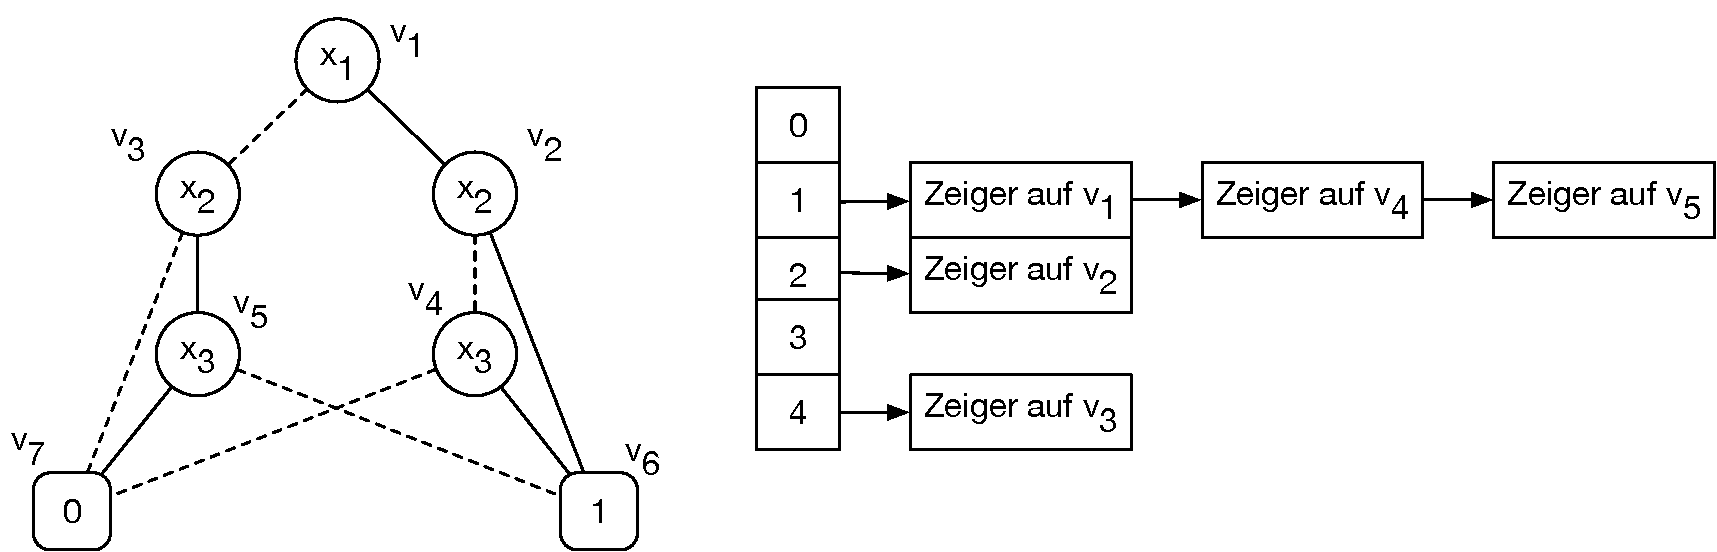
\includegraphics[scale=0.5]{./img/utable2}
	\caption[Verkettung von Überläufern]{Verkettung von Überläufern}
	\label{fig:verkettung}
\end{figure}\\
Die UT könnte insgesamt fünf Plätze umfassen, wobei eine Hashfunktion $h(x_i, v_j, v_k) = i + j + k$ $(mod$ $5)$ vorliegt. Für den Knoten $v_1$ gilt somit $1 + 2 + 3$ $(mod$ $5) = 1$, was den Hashwert kennzeichnet. Somit ordnet sich der Wert an Stelle $1$ im Feld ein. Allerdings hat $v_4$ bspw. ebenfalls diesen Hashwert. Aufgrund dieser Kollision wird der Zeiger auf diesen Knoten in eine Überläuferliste gespeichert. Unter der Annahme, dass das OBDD vor der Überprüfung reduziert war, gilt, dass eine Unterfunktion -- die durch das Tripel $(x_i, g, h)$ dargestellt wird -- genau dann bereits in dem OBDD existiert, wenn es einen Knoten in der Liste gibt, der das gleiche Tripel repräsentiert \cite[S.112-114]{mt1998}. Daraus folgt, dass es sehr leicht ist, den ROBDD auch während des Einfügens neuer Knoten aufrechtzuerhalten. Dementsprechend entfällt ein expliziter Aufruf von \texttt{reduce} (siehe Code \ref{lst:reduce} auf Seite \pageref{lst:reduce}).\\
Die Verkettung von Überläufern wurde bei diesem ROBDD-Paket dahingehend adaptiert, dass die Knoten $v_i$ direkt in die Liste abgelegt wurden, anstelle der Referenzen darauf. Hierzu wurde eine Komponente in Gestalt eines Vektors hinsichtlich der Datenstruktur gewählt, die einen Verweis auf den Knoten enthält, der den Nachfolger in der dazugehörigen Kollisionsliste darstellt. Wie bereits in Kapitel \ref{sec:knoten} auf Seite \pageref{sec:knoten} erwähnt, liegen die Knoten dadurch eng beieinander und durch ihre Position wird Zeiger-Arithmetik möglich, womit ein konstanter Zugriff auf alle Felder besteht. Die Annahme hierbei ist, dass das Finden eines Knotens in dem Vektor aufgrund des Lokalitätsprinzips schneller funktioniert, da der nächste Block darin gleichzeitig mit in den Cache geladen wird. Das Lokalitätsprinzip bezieht sich in diesem Zusammenhang auf die Zugriffswahrscheinlichkeit hinsichtlich einer Speicherzelle, d.\,h. dass die Wahrscheinlichkeit sehr hoch ist, dass diese auch in naher Zukunft wieder benötigt wird. Bei einer ursprünglichen verketteten Liste ist dieser Vorgang wesentlich schwieriger abzuschätzen, was von Zeigern bedingt wird.\\
Eine dementsprechende Evaluation ist im Kapitel \ref{sec:ovh} auf Seite \pageref{sec:ovh} ersichtlich.
\\\\
Wird die Gesamtlaufzeit der UTs (siehe Code \ref{lst:ite} auf Seite \pageref{lst:ite}) betrachtet, so beträgt diese bei einer erfolglosen Suche (Prüfung auf Nicht-Existenz sowie anschließender Eintragung des ROBDD-Knotens $v$ mit $l(v) = x_i$) durchschnittlich $O(\frac{n}{m})$ bezüglich der Schlüsselvergleiche. Die durchschnittliche Anzahl der Einträge der Überläuferliste entspricht $\frac{n}{m}$, wenn $n$ Elemente auf $m$ Listen verteilt werden. Diese entspricht dem Belegungsfaktor $a$ und der durchschnittlichen Suchzeit, wenn kein Erfolg vorhanden ist. Der jeweilige Knoten wiederum kann in $O(1)$ am Ende der Liste eingetragen werden.\\
Bei einer erfolgreichen Suche hingegen, wird die Laufzeit durch $O(1 + \frac{a}{2})$ konkretisiert, weil lediglich von Bedeutung ist, dass beim Einfügen eines $j$-ten Knotens die durchschnittliche Listenlänge $\frac{j-1}{m}$ besteht \cite[S.77]{h2002}.\\
In diesem Kapitel wurde beschrieben, wie eine UT funktioniert und wie eine damit zusammenhängende Hashfunktion gewählt werden muss, damit Knoten effizient gefunden werden können. Im nächsten Kapitel soll -- darauf aufbauend -- untersucht werden, inwieweit eine Kombination der UT und BDDs hinsichtlich der Datenstrukturen möglich ist.
\subsubsection{Kombination von UT und BDD}
\label{sec:utableBdd}
Anstelle der Benutzung von separaten ADTs für die UT und ROBDD-Knoten, können beide als Kombination aufgefasst werden. Somit existiert allgemein für jeden Knoten ein zusätzliches Feld, welches einen Verweis auf die Kollisionskette hat \cite{brb2007}. Dieser Zusammenhang wird von der Abbildung \ref{fig:cutableDag} wie folgt visualisiert:
\begin{figure}[bth]
	\centering
	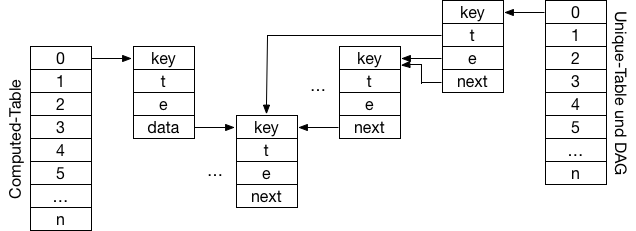
\includegraphics[scale=0.5]{./img/cutableDag}
	\caption[Kombination von UT und BDD]{Kombination von UT und BDD}
	\label{fig:cutableDag}
\end{figure}\\
\noindent
Hierbei steht DAG für einen gerichteten azyklischen Graphen (siehe Kapitel \ref{sec:bdd} auf Seite \pageref{sec:bdd}). Es werden zufällige Elemente im ROBDD in der Kollisionskette verbunden, was zur Folge hat, dass eine schnellere Ermittlung von Knoten im ROBDD stattfinden kann. Im Durchschnitt würde es hierbei nur noch vier Elemente pro Knoten geben. Dies impliziert eine Verbesserung des Speicherverhaltens, da der Overhead für die dazugehörige Allokation vermindert wird \cite{brb2007}. Wie bereits in Kapitel \ref{sec:utable} auf Seite \pageref{sec:utable} erwähnt, ist es jedoch auch möglich, das Feld \texttt{next} direkt in Vektoren abzulegen. Dadurch werden die Nachfolger in gemeinsame Slots abgelegt, wodurch sie nebeneinander liegen und ein Zugriff schneller erfolgen kann.\\
Um das Speicherverhalten genauer zu untersuchen, soll angenommen werden, dass sowohl die Computed-Table (siehe Kapitel \ref{sec:ctable} auf Seite \pageref{sec:ctable}) als auch die Kombination der UT/Knoten dieselben Speicherplätze benutzen. Der Ladefaktor von $4$ für die UT gewährleistet eine vertretbare gegenläufige Beziehung zwischen dem Auffinden eines Knotens in der Hashtabelle und dem dazugehörigen Overhead in Bezug auf den Speicher. Bei einem Ladefaktor von $4$ liegt die Speicherbenutzung somit bei ungefähr $22$ Bytes pro Knoten, wenn eine 64-Bit Maschine angenommen wird. Das Speicherverhalten geht aus den Experimenten in Kapitel \ref{sec:ovh} auf Seite \pageref{sec:ovh} genauestens hervor. Es werden dabei vier Wörter für jeden Eintrag in der Kombination von UT/Knoten benutzt, wobei drei Wörter den Schlüssel für eine Operation ausmachen, d.\,h. $f, g, h$ für $ite(f,g,h)$ (siehe Code \ref{lst:ite} auf Seite \pageref{lst:ite}) und ein Wort für das Resultat steht. So beschreiben $(f,g,h)$ den Block $(key, t, e, data)$ und $ite(f,g,h)$ den Block $(key, t, e, next)$. Zusätzlich kommen zwei Bytes als Overhead bezüglich des Speichers dazu.\\
Neben des effizienten Speicherns und der Wiederauffindung von Knoten innerhalb der Synthese (siehe Kapitel \ref{sec:ite} auf Seite \pageref{sec:ite}) wird im Folgenden die Implementierung des Caches beschrieben, womit ebenfalls die Performanz der Synthese gesteigert wird.

\subsection{Computed-Table}
\label{sec:ctable}
Um den Rechenaufwand bzw. Speicherplatz des ITE-Algorithmus (siehe Code \ref{lst:ite} auf Seite \pageref{lst:ite}) zu verringern, wird eine zweite Hashtabelle benutzt, die sog. \emph{Computed-Table} (CT). Diese Tabelle ist als Cache zu verstehen, d.\,h. bereits berechnete Ergebnisse werden dort abgespeichert, damit ein erneuter Zugriff in konstanter Zeit möglich bzw. der Gesamtaufwand bei den eben genannten Algorithmen polynomiell beschränkt ist, was im Folgenden diskutiert werden soll.\\
Bei der Beschreibung der Synthesen aus Kapitel \ref{sec:synthese} auf Seite \pageref{sec:synthese} werden sukzessive Operationen auf OBDDs angewendet. Bezüglich des ITE-Algorithmus wird mittels \texttt{cT.hasNext} geprüft, ob es bereits eine Zusammenstellung von betrachteten Operanden gibt, wobei im positiven Fall eine vorhandene Berechnung zurückgeliefert wird, was durch den folgenden Code \ref{lst:hasNext} verdeutlicht wird:
\lstset{language=xml}
\begin{lstlisting}[frame=htrbl, caption={Implementierung von {\ttfamily hasNext}}, label={lst:hasNext}]
program hasNext()
  input: key, node
  output: Status, ob es den Knoten bereits in der CT gibt
  pos := getKey(key)
  items := Paar mit Abbildungen von Keys auf Knoten
  if (key == items[pos].first) then
    node := items[pos].second
    return true
  end if
  return false
end program
\end{lstlisting}
Mithilfe von \texttt{cT.insert} wird wiederum eine solche Zusammenstellung sowie das berechnete Ergebnis gespeichert. Dementsprechend gilt hier \texttt{items[pos].first = key} und \texttt{items[pos].second = node} nach der Generierung des Schlüssels. Analog hierzu bildet der Cache drei Knoten $f,g,h$ auf den resultierenden Knoten $ite(f,g,h)$ ab. Somit können beim ITE-Algorithmus Rekursionsaufrufe eingespart werden, da bei den betrachteten Wegen -- von der Wurzel aus -- zu den Blättern isomorphe Teilgraphen nicht öfter betrachtet werden müssen. Damit verbundene Tests sind in Kapitel \ref{sec:vglcK} auf Seite \pageref{sec:vglcK} zu finden.\\
Hierbei ist ein ähnliches Problem zur UT erkennbar, das sich auf die Existenzprüfung sowie Speicherung von Ergebnissen in Form von Knoten bezieht, was im Best Case in $O(1)$ abläuft. Es ist daher unabdingbar, ebenfalls eine geeignete Wahl bezüglich der Hashfunktion sowie des Schlüssels (siehe Kapitel \ref{sec:hashing} auf Seite \pageref{sec:hashing}) zu treffen. Analog zur Funktion werden auch die darin benutzten Knoten $f, g$ bzw. $f, g, h$ benutzt. Hier kann dann ebenfalls entweder das Modulo- oder Multiplikationsverfahren angewendet werden.\\
Durch die Verwendung dieser Hashtabelle reicht somit bspw. bei \texttt{ite} eine Überprüfung aus, ob ein Tripel $(v_1, v_2, v_3)$ bereits auf einen Knoten $v$ zeigt, womit dieser dann wiederverwendet werden kann. Demzufolge muss lediglich erzielt werden, dass Rückschlüsse darauf gemacht werden können, für welche Operation ein Eintrag in der CT erzeugt wurde.\\
Im Gegensatz zur UT dürfen auch noch eventuell benötigte Knoten gelöscht werden, da hierdurch die Kanonizität nicht gefährdet wird. Es gibt also keine Notwendigkeit, Einträge bis zu ihrer Löschung zu speichern. Bezüglich der obigen Argumentation soll aufgrund der Effektivität auch kein Suchvorgang innerhalb der CT stattfinden. Um also Speicherplatz zu sparen, wird eine CT als sog. dynamischer \emph{hashbasierter Cache} eingesetzt (anfangs limitiert), d.\,h. es wird keine Kollisionsstrategie eingesetzt, was die Abbildung \ref{fig:uctable} auf Seite \pageref{fig:uctable} visualisiert:
\newpage
\begin{figure}[bth]
	\centering
	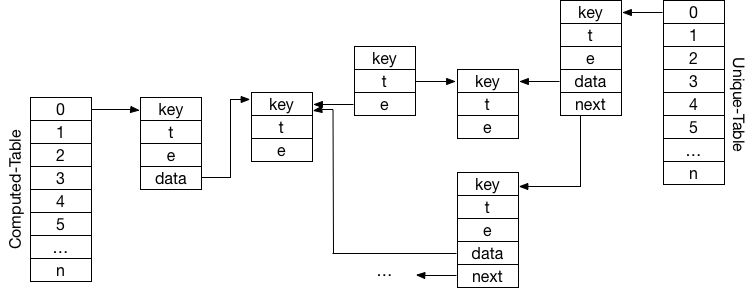
\includegraphics[scale=0.3]{./img/uctable}
	\caption[Zusammenhang zwischen Computed- und Unique-Table]{Zusammenhang zwischen Computed- und Unique-Table}
	\label{fig:uctable}
\end{figure}
Die zusammenhängenden Felder \textit{key}, \textit{t} und \textit{e} umschreiben dabei die jeweiligen Knoten im BDD. Um das Speicherverhalten dahingehend zu optimieren, werden UT und Knoten in einen ADT zusammengefügt. Diese Technik wird in Kapitel \ref{sec:utableBdd} auf Seite \pageref{sec:utableBdd} beschrieben.\\
Gibt es also bspw. bereits einen Eintrag für einen Knoten $v$ an einer Position $x$, so wird dieser Knoten durch einen anderen Knoten $v'$ überschrieben. Bezüglich des Ablaufs wird also zuerst die oberste Instanz einer Synthese abgefragt. Sollte hier seitens der CT keine positive Rückmeldung erfolgen, so besteht weiterhin die Chance, diese bei Subinstanzen zu bekommen. Empirische Studien zeigen, dass es häufig erfolglose Suchen gibt und daher die eben beschriebene Methode schneller als eine Suche hinsichtlich Überläuferlisten ist \cite[S.86]{h2002}. Im Gegensatz zu ROBDD-Knoten müsste dabei jeder Überläufer der CT zuerst den Speicherplatz der Stelle in der Liste allokieren, um anschließend Datensätze darin speichern zu können. Der größere Aufwand für eine solche Kollisionsstrategie wird also eingespart. Praktisch gesehen, kann es natürlich dennoch sein, dass die Synthese darunter leidet, da auch die Nachfolger für den überschriebenen Knoten nicht mehr in der CT enthalten sein müssen. So kann also bspw. die ITE-Operation nun im Worst Case eine exponentielle Laufzeit aufweisen, wenn alle Schlüssel auf denselben Wert bzw. Knoten zeigen. Dies ist jedoch in der Praxis kaum der Fall, sodass das Risiko praktisch eingegangen werden kann \cite{j2001}. Eine weitere Abhilfe schafft hierbei eine Approximation der Größe der CT. Empirische Resultate empfehlen hierzu insgesamt $500.000$ Einträge \cite[S.88]{h2002}. Experimente zwischen einem hashbasiertem Cache bzw. einem Cache mit Kollisionsstrategie unterstützen diese These, die in Kapitel \ref{sec:vglcK} auf Seite \pageref{sec:vglcK} ersichtlich sind.\\
Insgesamt sind also sowohl die Operation \texttt{hasNext} als auch \texttt{insert} offensichtlich in $O(1)$ möglich. Damit auch die Negation in konstanter Laufzeit ermöglicht wird, muss der Einsatz von komplementären Kanten erfolgen, die im nächsten Abschnitt erläutert werden.
\subsection{Komplementäre Kanten}
\label{sec:complementEdges}
In Kapitel \ref{sec:implementierung} auf Seite \pageref{sec:implementierung} wurde bereits angedeutet, dass die Verarbeitung der Negation nicht explizit durchgeführt werden muss, sondern mittels komplementärer Kanten in konstanter Zeit ermöglicht wird, anstelle von $O(|f|)$. Hierzu sollen die ROBDD-Knoten $f = x_0 \wedge x_1 \vee \neg x_0 \wedge x_2$ und $f' = x_0 \wedge \neg x_1 \vee \neg x_0 \wedge \neg x_2$ betrachtet werden:
\begin{figure}[bth]
	\centering
	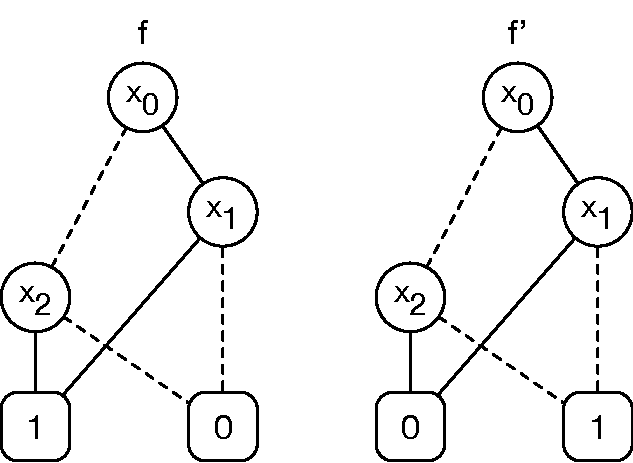
\includegraphics[scale=0.56]{./img/neg}
	\caption[Negation einer Funktion]{Negation einer Funktion}
	\label{fig:neg}
\end{figure}\\
\noindent
Bei einem Vergleich beider Darstellungen aus der Abbildung \ref{fig:neg} fällt auf, dass sie sich sehr ähnlich sind, wobei lediglich die $0$- und $1$-Blatt vertauscht sind. Formal werden die ON- und OFF-Menge (siehe Kapitel \ref{sec:bFunktionen} auf Seite \pageref{sec:bFunktionen}) vertauscht. Diese Erkenntnis kann dazu genutzt werden, festzulegen, wie die Markierung der Blätter interpretiert wird \cite{brb2007}. Der Knoten $f'$ wird demnach nicht gespeichert, sondern eine spezielle Kante auf $f$, die ein \emph{complement-Bit} gesetzt hat. Diese Kante wird als \emph{komplementäre Kante} (CE) bezeichnet und sagt aus, dass die Funktion -- in der diese Kante endet -- als komplementär interpretiert werden muss. Konkret wird also das Komplement einer Kante berücksichtigt, indem ein Bit in der Speicheradresse eines Knotens reserviert wird. Sollte es gesetzt sein, so wird das dazugehörige ROBDD als negiert interpretiert.\\
Wie bei herkömmlichen OBDDs (siehe Kapitel \ref{sec:ordnung} auf Seite \pageref{sec:ordnung}) ist die Auswertung derartig aufgebaut, dass der Berechnungspfad durchlaufen wird. Es wird jedoch zusätzlich gezählt, ob eine gerade oder ungerade Anzahl von Kanten mit der Markierung durchlaufen wird \cite[S.42-44]{h2002}. Sollte es eine ungerade Anzahl sein, so wird der Wert des jeweiligen erreichten Blattes negiert. Mit dieser beschriebenen Variante würde jedoch -- ohne weitere Regeln -- die Kanonizität verletzt werden, da sie nicht mehr bis auf Isomorphie eindeutig ist. So gibt es mehrere Fälle, wobei verschiedene Paare existieren, die jeweils funktional äquivalent zueinander sind \cite[S.119-121]{mt1998}. Wenn für einen Knoten $v$ das Tripel aus ausgehender high- und Low-Kante sowie eingehender Kante betrachtet wird, so gibt es genau $2^3 = 8$ Möglichkeiten, die Komplementbits zu setzen. Mithilfe der De Morganschen Gesetze (siehe Kapitel \ref{sec:formal} auf Seite \pageref{sec:formal}) kann diese funktionale Äquivalenz gezeigt werden:
\begin{equation*}
\begin{split}
\overline{x_if_{x_i} + \overline{x_i}f_{\overline{x_i}}} &= \overline{x_if_{x_i}} \cdot \overline{\overline{x_i}f_{\overline{x_i}}}\\
&= (\overline{x_i} + \overline{f_{x_i}}) \cdot (x_i + \overline{f_{\overline{x_i}}})\\
&= x_i\overline{f_{x_i}} + \overline{x_i}\overline{f_{\overline{x_i}}} + \overline{f_{x_i}}\overline{f_{\overline{x_i}}}\\
&= x_i(\overline{f_{x_i}} + \overline{f_{x_i}}\overline{f_{\overline{x_i}}}) + \overline{x_i}(\overline{f_{\overline{x_i}}} + \overline{f_{x_i}}\overline{f_{\overline{x_i}}})\\
&\overset{Absorption}{=} x_i\overline{f_{x_i}} + \overline{x_i}\overline{f_{\overline{x_i}}}\\
\end{split}
\end{equation*}
Diese Fälle bzw. vier Paare von Kombinationen zeigt die nachstehende Abbildung \ref{fig:complement}:
\begin{figure}[bth]
	\centering
	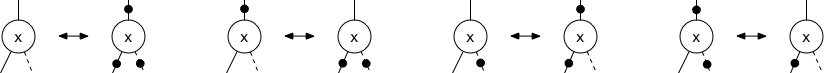
\includegraphics[scale=0.5]{./img/complement}
	\caption[Äquivalente Paare bei komplementären Kanten]{Äquivalente Paare bei komplementären Kanten}
	\label{fig:complement}
\end{figure}\\
\noindent
Hierbei stehen die schwarz gefärbten Kreise für sog. \textit{Output-Inverter}, womit die jeweiligen Kantenmarkierungen gekennzeichnet werden. So sind bspw. eine Kante zu einem $1$-Blatt und eine Kante mit Output-Inverter zu einem 0-Blatt äquivalent zueinander. Es bedarf also zusätzlicher Regeln für die Verwendung von Output-Invertern, um die Eindeutigkeit weiterhin sicherzustellen \cite[S.46-47]{s2007}:
\begin{enumerate}
	\item Es gibt nur noch ein 1-Blatt, wodurch ein Blatt also entfällt.
	\item Output-Inverter sind nur auf Low-Kanten erlaubt.
	\item Sollte ein OBDD eine Funktion $f$ darstellen, so gibt es i.\,d.\,R. auch einen Zeiger zu $f$, der auch einen Output-Inverter beinhalten darf. Andererseits würde sich ansonsten die konstante $0$-Funktion nicht als Komplement des $1$-Blattes darstellen lassen.
\end{enumerate}
\textbf{Hinweis:} Die ersten beiden Regeln können natürlich auch umgedreht werden. Wenn es also nur noch ein 0-Blatt gäbe, so würden Output-Inverter nur auf High-Kanten erlaubt sein.\\\\
Um also wieder für eine Eindeutigkeit zu sorgen, muss eine Eigenschaft ausgenutzt werden, die jeweils von den vier Paaren nur ein Bestimmtes erlaubt. Hier muss also bspw. die High-Kante immer regulär, d.\,h. nicht komplementär sein \cite[S.24-25]{s1997}. Sämtliche Regeln -- inklusive der Regeln aus Abbildung \ref{fig:reduktionen} auf Seite \pageref{fig:reduktionen} -- werden bei dem Aufruf von \texttt{findAdd} (siehe Code \ref{lst:ite} auf Seite \pageref{lst:ite}) angewendet, d.\,h. jedes OBDD wird weiterhin reduziert in der UT (siehe Kapitel \ref{sec:utable} auf Seite \pageref{sec:utable}) gespeichert:
\begin{enumerate}
	\item Eliminierung: Es wird im Fall $t=e$ die Speicheradresse von $t$ zurückgegeben.
	\item Isomorphie: Folgt automatisch aus der Konstruktion, da zwei verschiedene Knoten mit der gleichen ITE-Operation nicht gespeichert werden können.
	\item Negation: Gilt $t'$, so wird \texttt{res = findAdd(v, t', e')} gespeichert und \texttt{res} zurückgegeben.
\end{enumerate}
Alle OBDD-Operationen greifen lediglich nur mittels \texttt{findAdd} auf OBDD-Knoten zu. Somit erzeugen alle Operationen nur ROBDDs.\\
Die Abbildung \ref{fig:complementTransform} auf Seite \pageref{fig:complementTransform} zeigt dementsprechend nun die Überführung zweier ROBDDs ohne Output-Inverter für Boolesche Funktionen $f$ und $f'$ zu ROBDDs mit Output-Invertern:
\begin{figure}[bth]
	\centering
	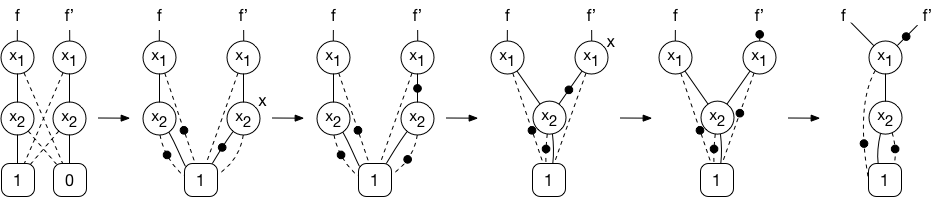
\includegraphics[scale=0.4]{./img/complementTransform}
	\caption[Überführung von ROBDDs zu ROBDDs mit Output-Invertern]{Überführung von ROBDDs zu ROBDDs mit Output-Invertern}
	\label{fig:complementTransform}
\end{figure}\\
\noindent
Gemäß der Abbildung \ref{fig:complementTransform} wird also zunächst das 0-Blatt entfernt, wobei alle eingehenden Kanten davon umgelenkt und komplementiert werden. Anschließend wird mittels einem Bottom-up Verfahren für jeden Knoten eine eindeutige Entscheidung zur Normierung der Kanten getroffen. Der betrachtete Knoten wir hier mit einem \textit{x} (siehe Abbildung) gekennzeichnet. Aufgrund der Kanonizität darf keine High-Kante einen Output-Inverter besitzen, weshalb $x_2$ normiert werden muss, d.\,h. die Marke wird entfernt und gemäß Abbildung \ref{fig:complement} auf Seite \pageref{fig:complement} (4. Fall) reduziert. Falls es möglich ist, so müssen ebenfalls die Reduktionsregeln der Isomorphie bzw. Redundanz angewendet werden. Analog dazu wird dieses Vorgehen für jeden Knoten durchgeführt. In der Praxis wird bereits bei der Konstruktion auf die Normierung geachtet, sodass eine nachträgliche Überführung nicht notwendig ist \cite[S.45]{h2002}.\\
Im Vergleich zu herkömmlichen OBDDs können letztendlich also mittels OBDDs mit CEs zu jedem Knoten $v$ zwei Funktionen dargestellt werden, nämlich $f_v$ und die dazugehörige Negation $f_v'$. Wenn $v$ also über eine Kante ohne Output-Inverter erreicht wird, so gilt $f_v$, ansonsten $f_v'$. Dadurch entstehen auch in Bezug auf den ITE-Algorithmus ein neuer Terminalfall, nämlich $ite(f, 0, 1) = f'$. Die Ausführung von Booleschen Operationen kann also durch die Ausnutzung von Regeln wie $f \cdot f' = 0$ oder $f + f' = 1$ beschleunigt werden.\\
Durch CEs lässt sich die Komplexität des ITE-Algorithmus demnach quadratisch beschränken, gdw. zwei der Argumente in jedem Aufruf komplementär sind \cite[S.119-121]{mt1998}. Für alle 16 binäre Operationen (siehe Tabelle \ref{tab:ite} auf Seite \pageref{tab:ite}) lässt sich dieses Kriterium anwenden, d.\,h. wenn es zwei OBDDs $G_a, G_b$ ($a, b \in \mathbb{B}_2$) mit CEs bezüglich einer Ordnung $\pi$ gibt, so kann das ROBDD $G'$ für $a \cdot b$ mit CEs mithilfe des ITE-Algorithmus in $O(|G_a||G_b|)$ bestimmt werden. Der zusätzliche Overhead, d.\,h. Verwaltungsaufwand von CEs bei ITE, ist als minimal zu bewerten \cite[S.19-22]{dfe2005}. Darüber hinaus wird kein zusätzlicher Speicher benötigt, wenn das niederwertigste Bit (LSB) von jedem Zeiger zur Kodierung des complement-Bits verwendet wird, was über die Bitmaske \texttt{(DDNode*) (ddNode \& ( (~( (size\_t) 0) >> 2) << 2) )} im Code abgefragt werden kann. Aufgrund dessen, dass alle gängigen Rechner nur gerade Adressen verwenden, entspricht dieses immer $0$ und kann demnach dafür benutzt werden. Um das Komplement anzuzeigen, kann also der Fakt ausgenutzt werden, dass Zeiger-Adressen ein Multiplikator von $4$ sind, weshalb die zwei niederwertigsten Bits genutzt werden, um Kanteninformationen zu erfassen. Die Not-Operation kann somit durch eine Kontravalenz mittels \texttt{(ddNode \^~complementEdge)} ausgedrückt werden. Das niederwertigste Bit davon wird wiederum für die Umkehrung benutzt. Im Best Case entspricht die Speicherplatzreduktion daher dem Faktor $2$, wofür die Paritätsfunktion (siehe Kapitel \ref{sec:dnfknf} auf Seite \pageref{sec:dnfknf}) ein gutes Beispiel ist \cite{brb2007}.\\
Arbiträre ROBDDs benötigen durchschnittlich $2n-1$ interne Knoten, wobei für \\ROBDDs mit CEs $n$ interne Knoten genügen. Auch die Abbildung \ref{fig:complementTransform} auf Seite \pageref{fig:complementTransform} zeigt darüber hinaus eine Knotenreduktion von 50 \%. Neben der Speicherplatzersparnis kann so auch leichter erreicht werden, dass der Speicherplatz für einen Knoten ein Teiler der Größe einer Cache-Zeile (kleinste Einheit zur Verwaltung im Cache von CPUs) ist \cite[S.47]{s2007}. Dieses Resultat kann konkret durch die eben angegebene Bitmanipulation erreicht werden, was eine verbesserte Performanz impliziert. Abschließend sei gesagt, wenn ein BDD mit CEs eingesetzt wird, so ist das ROBDD durchschnittlich 7 \% kleiner als ein herkömmlicher ROBDD, was durch Experimente in Kapitel \ref{sec:bddCom} auf Seite \pageref{sec:bddCom} beschrieben ist.\\
Neben den erläuterten CEs kann der ITE-Operator zudem dadurch verbessert werden, indem der Einsatz von Standard-Tripeln erfolgt. Im folgenden Kapitel soll daher deren Bedeutung erklärt werden.

\subsection{Standard-Tripel für ITE}
\label{sec:standard}
In Kapitel \ref{sec:ite} auf Seite \pageref{sec:ite} wurde der ITE-Operator diskutiert, indem unter anderem eine kubische bzw. quadratische Laufzeit bestimmt werden konnte. Darüber hinaus gibt es jedoch noch weitere Maßnahmen, um die Effizienz zu steigern, indem mehrdeutige ITE-Aufrufe hinsichtlich der Operanden für dieselbe Berechnung standardisiert werden.\\
Für den ITE-Operator gibt es Parameter $f_1, f_2, f_3$ und $g_1,g_2,g_3$, sodass $ite(f_1, f_2, f_3) = ite(g_1,g_2,g_3)$ gilt, wobei $\exists i : f_i \neq g_i$. Also kann auf der Menge von drei Funktionen $f_1, f_2, f_3$ bezüglich der Booleschen Funktion $ite(f_1, f_2, f_3)$ eine Äquivalenzrelation definiert werden, d.\,h. eine Relation, die reflexiv sowie symmetrisch und transitiv (siehe Kapitel \ref{sec:bFunktionen} auf Seite \pageref{sec:bFunktionen}) ist. Das Ziel dabei ist nun, Kombinationen von Operatoren -- die zum gleichen Ergebnis führen -- zu einer Äquivalenzklasse zusammenzufassen und einen Repräsentanten auszuwählen, der zur Durchführung einer ITE-Operation benutzt wird \cite[S.40]{h2002}.\\
Dadurch kann die Berechnung beschleunigt bzw. wiederholte Berechnungen vermieden werden. Weiterhin kann aber auch die CT (siehe Kapitel \ref{sec:ctable} auf Seite \pageref{sec:ctable}) klein bzw. effizient gehalten werden \cite[S.48]{s2007}. Wenn sich davon abstrahiert bspw. ein Eintrag $(v_1,v_2)$ bezüglich $\vee$ darin befindet, so sollte dieser auch gefunden werden, wenn ein Knoten für $(v_2,v_1)$ benötigt wird. Wie bereits in Tabelle \ref{tab:ite} auf Seite \pageref{tab:ite} gezeigt, können alle praktisch eingesetzten binären Operatoren mithilfe des ITE-Operators dargestellt werden. Demzufolge genügt in diesem Zusammenhang eine CT für diesen Operator.\\
Im Hinblick auf den ITE-Algorithmus (siehe Code \ref{lst:ite} auf Seite \pageref{lst:ite}) werden bei jedem Aufruf von $ite(f_1,f_2,f_3)$ zunächst die Standard-Argumente $g_1, g_2, g_3$ substituiert, bevor die Operationen \texttt{hasNext} bzw. \texttt{insert} bezüglich der CT aufgerufen werden. Die UT (siehe Kapitel \ref{sec:utable} auf Seite \pageref{sec:utable}) gewährleistet eine strenge Kanonizität, weiterhin werden CEs (siehe Kapitel \ref{sec:complementEdges} auf Seite \pageref{sec:complementEdges}) eingesetzt. Durch diese Methoden kann effizient bestimmt werden, ob zwei berechnete Boolesche Funktionen äquivalent sind \cite{brb2007}. Somit gilt bspw. $f + g \Leftrightarrow ite(f,f,g) = ite(f,1,g) = ite(g,1,f) = ite(g,g,f)$. Um das jeweilige \emph{Standard-Tripel} zu bestimmen, wird zunächst eine Umformung hinsichtlich der Parameter vorgenommen, wenn es möglich ist. Diese können wie folgt substituiert werden:
\begin{equation*}
\begin{split}
ite(f,f,g) &\Rightarrow ite(f,1,g)\\
ite(f,g,f) &\Rightarrow ite(f,g,0)\\
ite(f,g,f') &\Rightarrow ite(f,g,1)\\
ite(f,f',g) &\Rightarrow ite(f,0,g)
\end{split}
\end{equation*}
Hierbei kennzeichnet $f'$ eine CE. Um dementsprechend eine Umformung wie \\$ite(f,g,f') \Rightarrow ite(f,g,1)$ machen zu können, muss für zwei Funktionen effizient getestet werden, ob eine Funktion die Negation der anderen ist. Dies kann -- wie bereits beschrieben -- über CEs erfolgen.\\
Im Anschluss daran werden folgende Paare als Repräsentanten aus den Äquivalenzklassen benutzt:
\begin{equation*}
\begin{split}
ite(f,1,g) &\equiv ite(g,1,f)\\
ite(f,g,0) &\equiv ite(g,f,0)\\
ite(f,g,1) &\equiv ite(g',f',1)\\
ite(f,0,g) &\equiv ite(g',0,f')\\
ite(f,g,g') &\equiv ite(g,f,f')
\end{split}
\end{equation*}
Durch die Aufzählung aller möglichen Tripel für Operanden der Menge\\ $\{ f,f',g,g',h,h',0,1 \}$ lassen sich hierbei die Äquivalenzklassen bestimmen bzw. anschließend die eindeutigen Repräsentanten auswählen. Hinsichtlich der Implementierung werden beide Schritte in einer Funktion \texttt{standardize} als Code \ref{lst:standardize} zusammengefasst:
\lstset{language=xml}
\begin{lstlisting}[frame=htrbl, caption={Implementierung von {\ttfamily standardize}}, label={lst:standardize}]
program standardize()
  input: OBDD f, OBDD g, OBDD h, complementEdge
  output: Standardisierung
  // Identische Regeln
  if (f = g) then
    g := terminal(1)
  else if (f = h) then
    h := terminal(0)
  else if (f = !h) then
    terminal(1)
  else if (f = !g) then
    g := terminal(0)
  end if
  // Symmetrische Regeln
  if ( g = terminal(1) ) then
    if ( index(f) > index(h) ) then
      swap(f, h)
    end if
  else if ( g = terminal(0) ) then
    if ( index(f) > index(h) ) then
      swap(f, h)
      f = !f
      h = !h
    end if
  else if (g = !h) then 
    if ( index(f) > index(g) ) then
      swap(f, g)
      h = !g
    end if
  else if ( h = terminal(1) ) then
    if ( index(f) > index(g) ) then
      swap(f, g)
      f = !f
      g = !g
    end if
  else if ( h = terminal(0) ) then
    if ( index(f) > index(g) ) then
      swap(f, g)
    end if
  end if
  // CE-Regeln
  if ( isComplementEdge(g) ) then
    swap(g, h)
    f = !f
  end if
  if ( isComplementEdge(g) ) then
    g = !g
    h = !h
    complementEdge = !complementEdge
  end if
end program
\end{lstlisting}
Die Swap-Operation ist dafür zuständig, benachbarte Variablen zu vertauschen, wobei diese Prozedur eine lokale Operation kennzeichnet, in der nur die jeweiligen Knoten betrachtet werden, die mit diesen Variablen markiert sind. Um bspw. zwischen $ite(f,1,g)$ und $ite(g,1,f)$ den eindeutigen Repräsentanten zu bestimmen, wird das erste Argument mit der kleinsten top-Variable ausgewählt. Sollte es mehrere geben, so bestimmt der kleinste Adresszeiger der Knoten die Auswahl.\\
Wenn von CEs ausgegangen wird, so bestehen die Äquivalenzen \\$ite(f,g,h) = ite(f',h,g)$$= ite(f,g',h')' = ite(f',h',g')'$, wobei $f,g,h$ vereinfachte Parameter sind. Ein eindeutiger Repräsentant wird aus einem der vier Ausdrücke bestimmt, wobei -- damit übereinstimmend -- der ersten beiden Parameter von ITE keine CEs darstellen dürfen.\\
Diese Regeln können effektiv mithilfe der De Morganschen Gesetze (siehe Kapitel \ref{sec:formal} auf Seite \pageref{sec:formal}) bestimmt werden. Angenommen, $l$ und $h$ sind reguläre Kanten und es wird zunächst $l+h$ berechnet, so entsteht als Resultat $ite(l, 1, h)$. Wenn später $l' \cdot h'$, d.\,h. $ite(l',h',0)$ berechnet wird, so resultiert $ite(l,1,h)'$. Die CT hält also ein Resultat, was vor der Rückgabe lediglich komplementiert werden muss. Genauso können redundante Berechnungen wie z.\,B. $f+f' = ite(f,1,f') = ite(f,1,1) = 1$ ermittelt werden.\\
Neben den bisher erläuterten Techniken der Hashtabellen, komplementären Kanten und Standardtripeln zur Verbesserung des ITE-Algorithmus, soll im nächsten Abschnitt die Betrachtung der Knoten als Speicherblöcke erfolgen bzw. wie mit Knoten umgegangen werden soll, die für die ITE-Synthese nicht mehr benötigt werden.

\subsection{Die Speicherbereinigung}
\label{sec:speicherbereinigung}
Konkret betrachtet, entsprechen Knoten bzw. Kanten Speicherblöcken, wobei diese über Referenzen angesprochen werden können. Allerdings finden Manipulationen darauf in zufälligen Zugriffsmustern statt, die bei der Implementierung einer Speicherbereinigung beachtet werden müssen \cite[S.64]{h2002}. Grundsätzlich wird Speicher während der ROBDD-Anwendung den Knoten zugewiesen, damit sie manipuliert werden können. Wenn Knoten nicht mehr benötigt werden, so muss die Freigabe des Speichers erfolgen, damit diese Speicherstellen neu besetzt werden können. In diesem Zusammenhang muss der jeweilige eingesetzte Rechner bezüglich der Speicherverwaltung betrachtet werden.\\
Bei einer Computerarchitektur gibt es hinsichtlich der Speicherorganisation mehrere Komponenten, die im Hinblick auf die Größenordnung und Zugriffsgeschwindigkeit hierarchisch angeordnet sind:
\begin{figure}[bth]
	\centering
	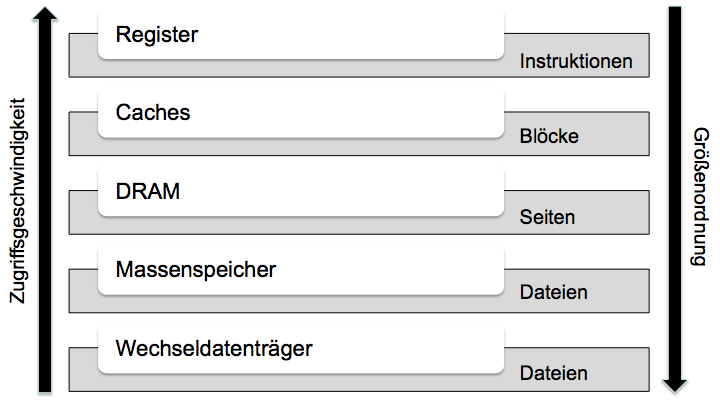
\includegraphics[scale=0.5]{./img/speicher}
	\caption[Die Speicherorganisation einer Computer-Architektur]{Die Speicherorganisation einer Computer-Architektur}
	\label{fig:speicher}
\end{figure}\\
\noindent
Eine Speicherhierarchie trägt maßgeblich dazu bei, dass Daten effizient gelesen bzw. geschrieben werden können. Wie anhand der Abbildung \ref{fig:speicher} auf Seite \pageref{fig:speicher} ersichtlich ist, wird die Performanz der Komponenten besser, je näher sich diese bei der CPU befinden, wobei auch dahingehend die Kosten steigen. Allerdings ist jedoch bspw. die Zugriffsgeschwindigkeit bei Caches wie dem Level-1-Cache (L1) oder Level-2-Cache (L2) schneller als beim Hauptspeicher. Die grundlegende Taktik sollte also sein, dafür Sorge zu tragen, dass wesentliche Inhalte als Kopien des DRAM in den Cache transferiert werden. Offensichtlich können somit auch Cache-Misses reduziert werden.\\
Die beschriebene Implementierung verfolgt den Ansatz einer automatischen Speicherbereinigung, wobei in den jeweiligen Konstruktoren (siehe Abbildung \ref{fig:class} auf Seite \pageref{fig:class}) mittels \texttt{new} Speicher allokiert bzw. mithilfe von \texttt{delete} in den Destruktoren dieser wieder freigegeben wird.\\
Wenn OBDDs konstruiert werden, so wird es häufiger vorkommen, dass berechnete Zwischenergebnisse nicht mehr benötigt werden, d.\,h. dass diese Knoten gelöscht werden können, womit auch die Nachfolger nicht mehr benötigt werden (insofern es nicht noch andere Zeiger darauf gibt). Um effizient zu ermitteln, ob ein Knoten noch benötigt wird, kann ein Zähler \texttt{id} für Referenzen realisiert werden. Jeder Knoten $v$ des Typs \texttt{DDNode} (siehe Kapitel \ref{sec:implementierung} auf Seite \pageref{sec:implementierung}) hat einen Referenzzähler als Indikator für die Anzahl der Referenzen auf $v$. Bei dessen Initialisierung gilt der Wert $1$. Um einen Overflow -- d.\,h. eine Überschreitung des darstellbaren Zahlenbereiches -- zu verhindern, gilt ein Maximum von $65535$ (umfasst zwei Bytes). Sollte dieses erreicht werden, so wird der Zähler beim späteren Löschen von Verweisen nicht wieder verringert. Der damit zusammenhängende Knoten würde also nicht mehr gelöscht werden, was einen Kompromiss zwischen der kompakten Darstellung und dem Speicherverbrauch ist. Sollte eine Formel bezüglich mehrerer aufgebauter Knoten freigegeben werden, so wird der Referenzzähler bei dem jeweiligen Knoten $f = (v,g,h)$ dekrementiert. Wenn der Zähler von $f$ dann~$0$ entspricht, so wird dieser Knoten als \emph{tot} markiert, andernfalls gilt er als \emph{lebendig}. Die Referenzzähler bei den Knoten $g,h$ werden diesbezüglich dann ebenfalls rekursiv verringert. Damit diese Prozedur automatisch erfolgen kann, wird der \texttt{DDNode} in den \texttt{BDDNode} eingehüllt. Somit erfolgt nicht nur eine automatische Inkrementierung der \texttt{id}, sondern auch eine automatische Dekrementierung. Der \texttt{BDDNode} hält also einen Zeiger auf den \texttt{DDNode} und es existiert eine bidirektionale Assoziation. In diesem Zusammenhang gibt es zwei Arten von Referenzzählern \cite[S.31]{s1997}:
\begin{itemize}
	\item \textbf{Interne Referenzzähler}: Sollte ein Wurzelknoten $r$ verwendet werden, so wird der interne Zähler von $r$ inkrementiert, um sicherzustellen, dass dieser nicht gelöscht werden kann. Wird hingegen $r$ an einer Stelle im SBDD (siehe Kapitel \ref{sec:sbdds} auf Seite \pageref{sec:sbdds}) nicht mehr benötigt, so erfolgt dementsprechend eine Inkrementierung.
	\item \textbf{Externe Referenzzähler}: Wenn eine Operation dem Anwender einen ROBDD zurückgibt, dann wird der externe Zähler inkrementiert. Dieser ist nun solange im Speicher vorhanden, bis der Anwender ihn explizit freigibt.
\end{itemize}
Die lebendigen Knoten werden dabei von der UT (siehe Kapitel \ref{sec:utable} auf Seite \pageref{sec:utable}) verwaltet. Wenn ein Knoten stirbt, so wird er demnach aus der Tabelle entfernt, indem der dazugehörige Speicher freigegeben wird. Die Effektivität der Speicherverwaltung wird im nächsten Kapitel \ref{sec:experimentelleErgebnisse} gezeigt.
